\documentclass[12pt]{article}

\usepackage[margin=2.5cm]{geometry}
\usepackage{times}
\usepackage{setspace}
\onehalfspacing

\usepackage[utf8]{inputenc}
\usepackage[T1]{fontenc}
\usepackage[romanian]{babel}
\usepackage{booktabs}

\usepackage{amsmath,amssymb,amsthm}
\usepackage{tikz-cd}
\usepackage{tikz}
\usepackage{multicol}
\usepackage{graphicx}
\usepackage{caption}
\usepackage{ragged2e}
\usepackage[hidelinks,hypertexnames=false]{hyperref}

\setlength{\parindent}{1.25cm}
\setlength{\parskip}{0pt}
\justifying
\emergencystretch=2em

\usepackage{titlesec}

\titleformat{\paragraph}
  {\normalfont\normalsize\bfseries}
  {\theparagraph}
  {1em}
  {}

\titlespacing*{\paragraph}
  {0pt}
  {1.25ex plus .2ex}
  {0.8ex}

\setcounter{secnumdepth}{4}
\setcounter{tocdepth}{4}

\numberwithin{equation}{section}
\numberwithin{figure}{section}
\numberwithin{table}{section}
\theoremstyle{definition}
\newtheorem{definitie}{Definiția}[section]
\newtheorem{observatie}{Observația}[section]
\theoremstyle{plain}
\newtheorem{propozitie}{Propoziția}[section]

\renewcommand{\figurename}{Figura}
\renewcommand{\tablename}{Tabelul}
\renewcommand{\contentsname}{Cuprins}
\renewcommand{\refname}{Bibliografie}

\newcounter{anexa}
\renewcommand{\theanexa}{\arabic{anexa}}
\newcommand{\anexasection}[2]{%
    \clearpage
    \refstepcounter{anexa}%
    \setcounter{figure}{0}%
    \setcounter{table}{0}%
    \renewcommand{\thefigure}{\theanexa.\arabic{figure}}%
    \renewcommand{\thetable}{\theanexa.\arabic{table}}%
    \section*{Anexă \theanexa: #1}%
    \addcontentsline{toc}{section}{Anexă \theanexa: #1}%
    \label{#2}%
}

\begin{document}
\setcounter{page}{1}
\pagestyle{empty}

\begin{titlepage}
    \begin{tikzpicture}[remember picture,overlay]
        \node[anchor=north west] at ([xshift=1.5cm,yshift=-1.5cm]current page.north west) {%
            \includegraphics[height=2.5cm]{logo-fmi.png}%
        };
        \node[anchor=north east] at ([xshift=-1.5cm,yshift=-1.5cm]current page.north east) {%
            \includegraphics[height=2.5cm]{logo-unibuc.jpg}%
        };
    \end{tikzpicture}

    \vspace{1.5cm}
    \centering

    {\Large Universitatea din București\\[0.1cm]}
    {\Large Facultatea de Matematică și Informatică\\[0.3cm]}
    {\large Specializarea Informatică\\[2.5cm]}

    {\Large\bfseries LUCRARE DE LICENȚĂ\\[1.2cm]}

    {\Huge\bfseries Aplicație de analiză a codului și asistență în generarea documentației proiectului: istoria structurală a codului la nivel de commit-uri, vizualizată drept graf interconectat\\[2.0cm]}

    \vfill

    \begin{flushleft}
        \large Coordonator științific: Conf. dr. Boriga Radu\\[0.4cm]
        \large Absolvent: Alexandrescu Andra
    \end{flushleft}

    \vfill

    {\large București\\}
    {\large iulie 2026}
\end{titlepage}

\section*{Rezumat}
\addcontentsline{toc}{section}{Rezumat}

Aplicația reprezintă un instrument de analiză și explorare a codului sursă al unui proiect, care extrage funcții dintr-un proiect, acestea fiind observate la nivel de commit-uri, prin intermediul parserelor arborilor de sintaxă (\textit{Abstract Syntax Tree, AST}~\cite{aho2006compilers}) specifice limbajelor TypeScript/ JavaScript, fiind observată structura codului, cât și evoluția temporală a conținutului. În cadrul acestei reprezentări, funcțiile extrase devin noduri într-un graf al proiectului, iar apelurile de funcții sunt definite prin muchii, reflectând astfel dependențele proiectului. De asemenea, aplicația combină un algoritm personalizat de PR (\textit{PageRank}~\cite{page1999pagerank}) pentru extragerea clusterelor relevante unei interogări în limbaj natural, asupra grafului de cunoștințe, cu generarea unei documentații prin metoda semisupervizată de învățare pe grafuri, DGI (\textit{Deep Graph Infomax}~\cite{velickovic2019dgi}). PR propagă relevanța semantică de la cel mai similar nod din punct de vedere semantic cu interogarea, de-a lungul dependențelor structurale, iar DGI are rolul de a produce embedding-uri ale nodurilor. În final pe baza acestora, clusterizarea ierarhică aglomerativă (\textit{Agglomerative Hierarchical Clustering}~\cite{ward1963hierarchical}), cu distanță cosinus și \textit{average linkage}, grupează entitățile în clustere de nivel superior și subclustere, constituind harta structurală a codului sursă. Astfel, utilizatorul poate vizualiza graful de dependințe, alături de evoluția cronologică a codului, având posibilitatea de a alege seed-urile PR și a le integra în documentația structurală generată de DGI, obținând un draft editabil.

\section*{Abstract}
\addcontentsline{toc}{section}{Abstract}

The application is a tool designed to analyze and explore a project's source code by extracting functions and examining them at the level of Git commits, using AST (\textit{Abstract Syntax Tree}~\cite{aho2006compilers}) parsers specific to TypeScript/ JavaScript, which enables to capture the code structure and its temporal evolution. Extracted functions become nodes in a project graph, while function calls are represented as edges, reflecting the project's dependencies. The application combines a custom PR (\textit{PageRank}~\cite{page1999pagerank}) algorithm to extract relevant clusters for a natural language query on the knowledge graph, with semisupervised graph based documentation generation via DGI (\textit{Deep Graph Infomax}~\cite{velickovic2019dgi}). PR propagates semantic relevance from the node that is most semantically similar to the query, along the structural dependencies, while DGI has the role of producing node embeddings. Based on these, agglomerative hierarchical clustering (\textit{Agglomerative Hierarchical Clustering}~\cite{ward1963hierarchical}) (using cosine distance and \textit{average linkage}) groups entities into higher level clusters and subclusters, constituting the structural map of the source code. Users can visualize the dependency graph and the code's chronological evolution, choose PR seed nodes and integrate them into the structural documentation generated by DGI, resulting in an editable draft.

\clearpage
\tableofcontents
\clearpage

\pagestyle{plain}

\section{Introducere}

\subsection{Subiectul lucrării}

Lucrarea propusă spre susținere pune accent pe inginerie software și metode de inteligență artificială aplicate codului sursă. Astfel, lucrarea aparține subdomeniilor instrumente pentru dezvoltatori (\textit{developer tools}), grafuri de cod (\textit{code knowledge graphs}), învățare automată pe grafuri (\textit{graph representation learning}).

Lucrarea abordează problema generării automate a unui graf de cunoștințe derivat din analiza codului sursă și a dependențelor dintre entitățile extrase, proximitatea semantică a acestora și evoluția lor temporală. Scopul este oferirea unei reprezentări, care este structurală, semantică și temporală, facilitând înțelegerea și navigarea unei baze de cod (codebase) de către o echipă de dezvoltare a proiectelor software.

\subsection{Motivația și formularea problemei}

În acest sens, motivația temei evidențiază necesitatea analizei evoluției unui proiect software, care nu poate fi redusă la o succesiune de commit-uri Git, deoarece commit-urile descriu modificări în contextul controlului de versiuni (\textit{version control}), dar nu reflectă structura logică a codului. Astfel, structura logică este definită prin dependențele structurale și semantice dintre funcții și module, fiind oferită o perspectivă esențială pentru organizarea și colaborarea unei echipe de dezvoltare. În plus, este necesară și o abordare semantică, prin soluții de căutare semantică la nivel de cod. De aceea, tema este relevantă: unificarea celor trei perspective într-un singur instrument poate reduce fragmentarea fluxurilor de lucru ale dezvoltatorilor.

\subsection{Metoda propusă}

Așadar, soluția propusă unifică cele trei niveluri într-un cadru coerent, în loc să le trateze ca module independente. Astfel, codul sursă este transformat într-un graf de cunoștințe prin analiză statică bazată pe parsere AST (\textit{Abstract Syntax Tree}~\cite{aho2006compilers}), unde nodurile extrase reprezintă entități de tipul funcțiilor și metodelor, iar muchiile descriu dependențe statice, precum apeluri directe, referințe și importuri. Acest strat structural este completat de un strat temporal, obținut din istoricul Git, unde, pentru fiecare commit, se analizează fișierele adăugate, modificate sau șterse și se urmărește evoluția entităților în timp. Spre deosebire de abordările care atașează separat un motor de căutare semantică~\cite{husain2019codesearchnet}, înțelegerea semantică este integrată direct în graf prin reprezentări învățate: metoda semisupervizată DGI (\textit{Deep Graph Infomax}~\cite{velickovic2019dgi}), bazată pe o rețea convoluțională pe grafuri (\textit{Graph Convolutional Network}, GCN), produce embedding-uri care surprind atât proximitatea structurală, cât și coerența funcțională a nodurilor. Aceste reprezentări permit atât interogări în limbaj natural prin propagarea relevanței în graf cu un algoritm PR (\textit{PageRank}~\cite{page1999pagerank}), cât și clusterizarea automată a subgrafurilor tematice, realizată prin clusterizare ierarhică aglomerativă (\textit{Agglomerative Hierarchical Clustering}~\cite{ward1963hierarchical}) pe embedding-urile DGI. Rezultatul este o sugestie structurată de documentație: grupări funcționale identificate algoritmic, bazate pe relațiile dintre entități și evoluția lor temporală.

\section{Preliminarii}

\subsection{Noțiuni fundamentale}

Conceptele abordate în această lucrare sunt analiza statică a codului, reprezentarea grafică a dependențelor, căutarea semantică și învățarea pe grafuri. În cele ce urmează sunt prezentate noțiunile teoretice care stau la baza soluției propuse.

Arborele de sintaxă (\textit{Abstract Syntax Tree}, AST~\cite{aho2006compilers}) este o reprezentare ierarhică a structurii sintactice a unui program, în care nodurile reprezintă construcții de cod, iar muchiile relațiile dintre ele.

Căutarea semantică a codului (\textit{Semantic Code Search}~\cite{husain2019codesearchnet}) identifică fragmente relevante pe baza semnificației, nu a unei potriviri textuale.

\textit{PageRank} (PR)~\cite{page1999pagerank} ordonează nodurile unui graf orientat modelând un utilizator care urmează muchiile cu o anumită probabilitate și sare la un nod ales la întâmplare (\textit{teleportare}).

O rețea convoluțională pe grafuri (\textit{Graph Convolutional Network}, GCN~\cite{kipf2017gcn}) actualizează reprezentarea fiecărui nod prin agregarea informației de la vecinii săi.
\textit{Deep Graph Infomax} (DGI)~\cite{velickovic2019dgi} este o metodă nesupervizată de învățare pe grafuri care antrenează un encoder GCN astfel încât fiecare nod să fie aliniat cu un sumar global al grafului, discriminatorul distingând perechile reale de cele corupte. În lucrare, DGI este extins semisupervizat pe perechi nod-limbaj natural.

Clusterizarea ierarhică aglomerativă (\textit{Agglomerative Hierarchical Clustering}~\cite{ward1963hierarchical}) fuzionează iterativ cele mai apropiate clustere, pornind de la noduri individuale (\textit{bottom-up}).

\subsection{Stadiul actual al subdomeniului}

Abordările existente acoperă, în general, doar două dintre cele trei niveluri de abstractizare relevante pentru înțelegerea unui proiect software: cel \textit{temporal} (istoricul modificărilor) și cel \textit{structural} (dependențele dintre entități). Nivelul \textit{semantic} este tratat de regulă separat, prin soluții de căutare semantică a codului (\textit{Semantic Code Search})~\cite{husain2019codesearchnet}, care combină LLM-uri și embedding-uri vectoriale. Modele precum \textbf{CodeBERT}~\cite{feng2020codebert} și \textbf{UniXcoder}~\cite{guo2022unixcoder}, antrenate pe cod sursă, obțin rezultate bune la similitudinea între fragmente de cod, dar alinierea cod, limbaj natural rămâne dificilă.

Platformele comerciale extind această direcție spre agenți și interogări în limbaj natural: \textbf{Sourcegraph}~\cite{sourcegraph2026} oferă căutare semantică la scară de codebase și context pentru agenți prin MCP, \textbf{Sonde}~\cite{sonde2026} construiește un graf structural cu integrare \textbf{Git} și analiză temporală,  iar \textbf{Pieces Desktop}~\cite{pieces2026} oferă memorie pe termen lung a fluxului de lucru și căutare conversațională, tot prin MCP. În literatura de cercetare, au fost propuse și metode care integrează căutarea semantică cu grafuri de apeluri și GCN ~\cite{abadsieper2020semantic}, însă fără o abordare care să includă integrarea Git sau generarea documentației unui proiect.

Reprezentările pe grafuri (\textit{Node2Vec}, \textit{GNN}, \textit{DGI}) îmbunătățesc modelarea relațiilor dintre entități, dar puține soluții software le combină cu sincronizarea \textbf{Git}, explorarea istoricului codului și un flux coerent de documentare automată. Așadar, lucrarea de față unifică nivelul temporal, structural și semantic într-o aplicație.

\begingroup
\sloppy
\section{Analiza și proiectarea sistemului}

Alegerea acestor tehnologii este determinată de caracterul \textit{local-first}~\cite{kleppmann2019localfirst} al aplicației și al necesității accesului controlat la sistemul de fișiere. Astfel, cerința de a integra procese de analiză software cu metode de învățare automată necesită stocarea pe calculatorul utilizatorului. Limbajele de programare folosite sunt \textbf{TypeScript}, rulat pe \textbf{Node.js} (pentru interfață, API, orchestrare desktop și analiză statică a codului sursă) și \textbf{Python} (pentru componentele de învățare automată: preprocesarea grafurilor, embedding-uri \textbf{UniXcoder}, antrenarea și inferența \textit{DGI}, clusterizarea prin \textit{PageRank} personalizat și generarea documentației structurale).

\subsection{Interfață utilizator}

Partea de frontend este construită cu framework-urile \textbf{Next.js} și \textbf{React}, în timp ce stilizarea este realizată cu \textbf{Tailwind CSS}.

În plus, componentele interfeței precum formularele de autentificare, înregistrare, creare proiect și configurare credențiale GitHub sunt gestionate prin \textbf{React Hook Form}, cu validare declarativă definită în scheme \textbf{Zod 4}.

Vizualizarea grafului de cunoștințe se bazează pe biblioteca \textbf{reagraph}~\cite{reagraph2026}, a cărei randare se face în \textbf{WebGL}, nu prin SVG sau DOM, nodurile și muchiile fiind vizualizate eficient pe un canvas, ceea ce permite navigarea fluentă în grafuri cu multe entități. Există limitări, fiind suficiente operații pe GPU care depind de complexitatea grafului proiectului, motiv pentru care încărcarea vizualizării și a interacțiunilor în canvas este influențată direct. În plus, afișarea codului sursă din commit-uri în mod cronologic se bazează pe \textbf{react-syntax-highlighter}, care aplică evidențiere (\textit{syntax highlighting}) prin motorul dedicat evidențierii sintactice numit Prism, inferând limbajul de programare automat din extensia fișierului.

\subsection{Mediu de execuție desktop}

Shell-ul aplicației este realizat cu \textbf{Electron}, care conține interfața web și oferă acces la operațiile native necesare unei aplicații de analiză a codului: selectarea directoarelor de proiect pentru citire și scriere, lansarea proceselor de analiză și gestionarea datelor locale.

La acest nivel sunt prezente servicii auxiliare, iar acestea au rolul de a comunica cu \textbf{GitHub}, de aceea sunt folosite platformele \textbf{cloudflared} pentru expunerea temporară a serviciilor locale către internet și \textbf{Azure Functions} care primește webhook-uri \textbf{GitHub}.

\subsection{Persistența datelor}

De asemenea, deși aplicația urmează un model \textit{local-first}, este necesar un strat de coordonare via \textbf{PocketBase}, care rulează local și este un backend ușor, cu o bază de date \textbf{SQLite} încorporată. \textbf{PocketBase} gestionează conturile utilizatorilor și sesiunile, înregistrările de proiect, credențialele \textbf{GitHub} (token, secret webhook), evenimentele recepționate de la \textbf{GitHub} și partajările între utilizatori. Aceste date trebuie să fie accesibile atât API-ului local, cât și serviciului \textbf{Azure Functions} (prin tunel), spre deosebire de fișierele de dimensiuni mari, care rămân stocate local, exemplu fiind grafurile, embedding-urile, snapshot-urile de commit-uri și documentațiile care se află în folder-ul de sistem AppData.

\subsection{Integrarea cu GitHub}

Integrarea cu \textbf{GitHub} este realizată prin \textbf{GitHub REST API} și \textbf{Azure Functions}. Această componentă permite aplicației să primească evenimente de tip \textbf{git push}, să valideze autenticitatea acestora și să sincronizeze informațiile relevante despre commit-uri.

Pe lângă integrarea prin API, sistemul utilizează și \textbf{Git} local pentru operații de tip \textbf{git pull} în directorul proiectului. Astfel, este posibilă menținerea unei copii locale actualizate a codebase-ului și facilitează corelarea modificărilor \textbf{Git} cu entitățile extrase prin analiza statică.

\subsection{Analiză statică a codului sursă}

Extragerea entităților funcționale și a dependențelor structurale se realizează prin parsarea codului sursă TypeScript și JavaScript cu \textbf{ts-morph}~\cite{tsmorph2025}, bibliotecă care oferă acces programatic la \textit{AST}, fără a utiliza language server-ul TypeScript/ JavaScript \textbf{tsserver}, ci constituie un strat de abstracție peste TypeScript Compiler API. Alegerea acestei soluții este motivată de faptul că analiza abordată în această lucrare se referă la proiectele dezvoltate în limbajele TypeScript și JavaScript. O extindere către mai multe limbaje de programare ar impune fie adoptarea unui language server dedicat fiecărui limbaj, fie implementarea manuală a mecanismelor de rezolvare a apelurilor între fișiere (\textit{cross-file calls}), adaptate la particularitățile fiecărui parser și modulele fiecărui limbaj. De aceea, analiza statică a codului este limitată la TypeScript/ JavaScript.

\subsection{Învățare automată pe grafuri}

Reprezentările semantice și operațiile de clusterizare sunt implementate în Python, folosind \textbf{PyTorch}~\cite{paszke2019pytorch} și \textbf{PyTorch Geometric}~\cite{fey2019fast} pentru reprezentarea grafului și antrenarea encoderului \textit{GCN}, \textit{Deep Graph Infomax} (DGI) pentru embedding-uri sensibile la topologie, \textbf{UniXcoder} (prin Hugging Face Transformers) pentru codificarea inițială a nodurilor, \textbf{scikit-learn}~\cite{pedregosa2011sklearn} pentru clusterizare ierarhică aglomerativă și similaritate cosinus, și \textit{PageRank personalizat} pentru identificarea subgrafurilor relevante unei interogări în limbaj natural.

\endgroup

\section{Implementare}

\subsection{Analiza codului sursă și construirea grafului structural}

\subsubsection{Configurarea}

În contextul analizei unui proiect, este necesară selectarea de către utilizator a folder-ului care conține codul sursă al repository-ului local. Astfel, selectarea căii via mecanimsul IPC al shell-ului Electron implică o asociere între utilizator și calea proiectului stocată într-un fișier de setări al aplicației, astfel încât alte analize ulterioare și sincronizarea commit-urilor să poată fi realizate fără reselectarea folderului.

\subsubsection{Extragerea entităților, nodurilor, muchiilor și dependențelor}

În continuare, parcurgerea codului sursă este realizată recursiv din calea proiectului, iar acest fapt presupune identificarea tuturor fișierelor TypeScript și JavaScript, fiind excluse folderele de dependențe, build, control de versiune și medii virtuale.
Astfel, fiecare fișier este transformat într-un arbore \textit{Abstract Syntax Tree}~\cite{aho2006compilers}, iar din acesta se extrag entități și relații între acestea.

Din arborii sintactici obținuți se extrag, în cadrul aceleiași analize, atât nodurile grafului, cât și muchiile dintre ele. Nodurile corespund funcțiilor de nivel superior (\textit{export function}), metodelor din clase și expresiilor funcționale (\textit{arrow functions} sau funcții anonime atribuite variabilelor), iar pentru fiecare astfel de entitate se rețin identificatorul unic derivat din calea și poziția din fișier a funcției, tipul și numele, cât și conținutul funcției, deoarece aceste informații sunt utilizate ulterior la generarea embedding-urilor semantice.

Referitor la relațiile care se stabilesc între entități, muchiile exprimă dependențe statice din cod, fără executarea acestuia. Astfel, este parcurs corpul fiecărei entități și sunt identificate relațiile cu alte funcții. Există două categorii de muchii extrase, deoarece este necesară o diferență de abordare pentru stabilirea relațiilor între entități. Muchiile de tip apel (\textbf{CALLS}) corespund invocărilor directe ale funcțiilor, fie în același fișier, fie între fișiere diferite, precum și utilizării componentelor React în JSX, deoarece acestea sunt interpretate ca invocări ale funcțiilor care definesc componentele respective. Muchiile de tip utilizare (\textbf{USES}) surprind referințe la alte funcții fără apel imediat, cum ar fi transmiterea unui callback ca argument sau folosirea unei funcții ca middleware. În aceeași categorie intră și dependențele din fișierele care importă module prin \textit{require}, deoarece legătura se stabilește prin utilizarea numelui importat în cod, nu printr-o expresie de apel cu paranteze, iar rezolvarea simbolică TypeScript dată de librăria ts-morph omite acest caz.

\subsubsection{Post-procesare, vizualizare și persistență}

Graful brut obținut după inferența muchiilor poate conține noduri fără nicio legătură cu restul rețelei, acest fapt însemnând că există funcții extrase din \textit{AST} niciodată apelate sau referențiate. Aceste noduri izolate sunt eliminate în etapa de post-procesare, deoarece nu contribuie la înțelegerea structurii dependențelor.

În interfață, graful este transformat într-o structură de vizualizare prin intermediul \textbf{reagraph} și grupează nodurile după fișier, separă muchiile în apeluri \textit{in-file} și \textit{cross-file} și calculează componentele conexe posibile. În plus, partiționarea în componente conexe este o măsură de gestionare a complexității, însemnând că în mod implicit, interfața afișează o singură componentă, permițând utilizatorului să navigheze între subgrafuri disjuncte ale codebase-ului, astfel evitând supraîncărcarea randării la scară mare.

Fișierul final conține graful structural complet, statisticile analizei și metadatele de vizualizare, împreună cu calea rădăcină a proiectului analizat.

Interfața canvasului care conține graful de cunoștințe este ilustrată în Figura~\ref{fig:knowledge-graph-interface} din Anexa~\ref{anexa:interfata-aplicatie}.

\subsection{Integrarea GitHub, sincronizarea commit-urilor și dimensiunea temporală a grafului}

Interfața paginii dedicate commit-urilor GitHub, folosită pentru inspectarea evenimentelor primite de aplicație de la GitHub, este prezentată în Figura~\ref{fig:webhook-events-interface} din Anexa~\ref{anexa:interfata-aplicatie}.

\subsubsection{Credențiale GitHub și înregistrarea webhook-ului}

Conectarea la \textbf{GitHub} se realizează din interfață, unde utilizatorul care deține proiectul completează un formular cu tokenul \textbf{GitHub} de acces personal, numele owner-ului și al repository-ului. Astfel, datele sunt validate și transmise către API-ul aplicației, care le stochează în \textbf{PocketBase} sub forma unei înregistrări de credențiale asociate utilizatorului și proiectului.

Folosind token-ul utilizatorului, serverul creează pe \textbf{GitHub} un webhook care verifică evenimentele de tip \textit{push} și \textit{pull request}, direcționate către funcția \textbf{Azure}. Deoarece funcția care primește evenimente GitHub, existentă în \textbf{Azure Functions}, este expusă public, server-ul generează un secret de webhook și îl salvează împreună cu token-ul în \textbf{PocketBase}, precum și în configurația webhook-ului de pe GitHub, pentru a putea verifica autenticitatea evenimentelor primite. Astfel, de fiecare dată când are loc o acțiune asupra repository-ului, GitHub semnează payload-ul cu acest secret, iar funcția Azure validează semnătura înainte de procesare, astfel încât doar evenimentele autorizate sunt acceptate.

După validare, funcția identifică proiectul și utilizatorul după owner-ul și numele repository-ului, consultând credențialele stocate în PocketBase, apoi redirecționează evenimentul către API-ul local al aplicației, accesibil prin tunelul \textbf{cloudflared}. În cazul în care validarea repository-ului sau crearea webhook-ului eșuează, înregistrarea credențialelor este anulată, astfel încât proiectul să nu rămână într-o stare parțial configurată.

\subsubsection{Evenimente webhook, sincronizarea commit-urilor și actualizarea folder-ului local}

În continuare, la primirea unui eveniment de tip \textit{push}, backend-ul normalizează payload-ul în înregistrări individuale de tip commit și le salvează într-o colecție de evenimente webhook, evitând duplicatele pentru același SHA. Pentru fiecare commit nou, serverul interoghează API-ul GitHub pentru lista fișierelor adăugate, modificate sau șterse, apoi salvează conținutul local, împreună cu un fișier numit \textbf{manifest.json} care reține metadate despre conținutul fiecărui commit.

În interfață, commit-urile sunt listate din evenimentele webhook stocate în \textbf{PocketBase}. Sincronizarea suplimentară cu GitHub, care este declanșată la deschiderea proiectului sau la solicitarea explicită a utilizatorului, are rolul de recuperare și completare a istoricului. În general acest fapt este necesar în două situații: la prima configurare a credențialelor, când istoricul preexistent trebuie importat din GitHub, și la repornirea aplicației, când commit-urile produse în absența tunelului \textbf{cloudflared} sau a funcției \textbf{Azure} nu au putut fi receptate în timp real, atunci când aplicația nu rulează. Așadar, înregistrările din PocketBase sunt completate în final, iar fișierele lipsă sunt exportate în folder-ul de commit-uri din \textbf{AppData}.

În timpul rulării aplicației, commit-urile sunt receptate prin webhook-uri, ce presupune că fiecare eveniment este înregistrat în PocketBase, iar fișierele asociate sunt exportate local. În plus, se realizează o verificare periodică cu GitHub atunci când un eveniment nu a fost livrat, însemnând că webhook-ul nu a funcționat temporar chiar dacă aplicația rulează. În cazul în care astfel de commit-uri noi sunt detectate în timp ce utilizatorul vizualizează proiectul, interfața solicită actualizarea folder-ului sursă al proiectului printr-un \textit{git pull} executat de shell-ul Electron, astfel încât analiza structurală ulterioară să reflecte codul actualizat alături de evenimentele webhook recepționate.

\subsubsection{Analiza temporală a funcțiilor și integrarea istoricului în graf}

Analiza codului sursă este realizată din interfața grafului de cunoștințe prin IPC-ul shell-ului Electron și este executat script-ul de analiză cu extragerea entităților asupra folder-ului proiectului configurat.

În cadrul aceleiași execuții, script-ul realizează mai întâi analiza structurală a proiectului întreg, descrisă în secțiunea anterioară și salvează rezultatul. Ulterior, dacă există directoare de commit-uri în \textbf{AppData}, acestea sunt procesate cronologic, iar pentru fiecare commit se parsează doar fișierele adăugate sau modificate. Urmează ca din fișierele parsate să fie extrase funcțiile, iar pentru a  stabili modificările asupra fiecărei funcții, script-ul le compară cu lista completă a funcțiilor întâlnite în commit-urile procesate anterior, marcându-le ca adăugate, modificate sau șterse. La final, toate modificările înregistrate per commit sunt combinate într-un fișier care reține istoricul fiecărei funcții.

Astfel, în cadrul vizualizării grafului de cunoștințe, istoricul fiecărei funcții este adăugat ca metadată, fără a modifica muchiile sau topologia grafului. Așadar, nodurile își schimbă culoarea în funcție de ultima modificare înregistrată (\textbf{added}, \textbf{modified}, \textbf{removed}), iar la selectarea unui nod utilizatorul poate consulta istoricul commit-urilor asociate. În plus, un subgraf separat ilustrează funcțiile șterse definitiv din codebase, completând evoluția istorică a proiectului.

\subsection{Procesarea semantică: embedding-uri, DGI, căutare PR și generarea documentației}

\subsubsection{Arhitectura generală}

Procesarea semantică a grafului de cunoștințe este organizată în diferite etape, fiind folosită arhitectura modelului \textit{Deep Graph Infomax}~\cite{velickovic2019dgi}. Stratul de pre-procesare produce, pentru fiecare proiect, un fișier care îmbină vectorii \textbf{UniXcoder} ai nodurilor cu structura \textbf{PyTorch Geometric} a grafului, iar acest strat este necesar atât pentru antrenarea modelelor, cât și pentru inferența din interfață. Stratul de antrenare, executat în afara fluxului din aplicație, antrenează encoderul \textit{DGI} în mod nesupervizat pe un corpus limitat de proiecte, apoi îl antrenează suplimentar supervizat pe perechi formate din interogări și noduri. Stratul de inferență este expus în interfața grafului de cunoștințe și folosește două reprezentări diferite: căutarea de clustere de noduri prin \textit{PR}, care operează în spațiul brut \textbf{UniXcoder}, cu proiecția interogărilor în limbaj natural și generarea documentației, care utilizează embedding-urile rafinate \textit{DGI}.

\subsubsection{Pre-procesarea grafului și generarea embedding-urilor}

Înainte de orice operație semantică, frontend-ul verifică prin endpoint-ul corespunzător dacă graful proiectului conține embedding-urile necesare etapelor de antrenare sau inferență, iar în cazul în care fișierul ce conține preprocesarea grafului unui proiect nu există, server-ul execută un script, care calculează embedding-urile \textbf{UniXcoder} pentru fiecare funcție, le cache-uiește și construiește structura \textbf{PyTorch Geometric} a grafului, salvând rezultatul final.

Așadar, script-ul citește fișierul de analiză \textit{AST} a grafului și încărca modelul \textbf{UniXCoder} (\textbf{microsoft/unixcoder-base}~\cite{guo2022unixcoder}), ales în locul \textbf{CodeBERT}~\cite{feng2020codebert}, deoarece separă mai bine conținutul funcțiilor distincte în spațiul vectorial. Într-un stadiu anterior al lucrării, s-a comparat distribuția similarității cosinus între perechi aleatoare de funcții din același proiect, pentru \textbf{CodeBERT} și \textbf{UniXcoder}. \textbf{CodeBERT} a produs valori medii mult mai ridicate, însemnând că embedding-urile funcțiilor diferite erau frecvent foarte apropiate în spațiul vectorial. În acest caz, pentru un graf de cunoștințe, căutarea semantică nu ar descoperi noduri relevante, deoarece funcțiile distincte primesc reprezentări aproape identice. \textbf{UniXcoder} a obținut o similaritate medie mai scăzută între perechi oarecare, indicând un spațiu mai bine separat. Dintr-o perspectivă teoretică, \textbf{CodeBERT} este antrenat prin masked language modeling pe cod sursă, fără aliniere explicită între limbaj natural și cod, în timp ce \textbf{UniXcoder} folosește pre-antrenare multimodală, incluzând perechi cod-comentariu și învățare contrastivă, astfel încât reprezentările să capteze atât semantica funcțională, cât și structura sintactică.

În continuare, pentru fiecare nod, codul sursă al funcției este encodat într-un vector de 768 de dimensiuni. Această valoare corespunde dimensiunii de ieșire a arhitecturii folosite de \textbf{UniXcoder}. Deoarece modelul \textbf{UniXcoder} acceptă o intrare limitată la 512 de tokeni, funcțiile ale căror cod sursă depășește această lungime sunt segmentate cu o suprapunere de 128 de tokeni între segmente adiacente, pentru a evita pierderea contextului. Astfel, fiecare segment produce un vector de reprezentare, iar embedding-ul final al funcției se obține prin medierea acestor vectori parțiali. Rezultatele sunt memorate în cache, sub formă de fișiere \textbf{.npy}, în contextul evitării recalculării la rulări ulterioare ale pre-procesării. Graful este transformat într-un graf neorientat deoarece relația dintre muchii nu oferă informație relevantă la nivel de învățare automată. Într-un final, rezultatul final este stocat local, cu extensia \textbf{.pkl}, conținând matricea de caracteristici, lista nodurilor cu muchiile neorientate și embedding-urile funcțiilor.

\subsubsection{Antrenarea reprezentărilor DGI}

Antrenarea modelelor nu este declanșată din interfața utilizatorului, ci constituie o fază de pregătire a corpus-ului. Antrenarea a fost realizată pe un corpus limitat de 67 de proiecte, cu un număr de 11420 fișiere analizate, având un total de 25935 noduri și 136129 de muchii identificate. Inițial, abordarea a fost transductivă, care ar fi cerut reantrenare la fiecare proiect nou, dar în implementarea finală este antrenat un encoder de graf inductiv, ce presupune o funcție cu ponderi învățate pe corpus-ul de antrenare și refolosite la inferență.

În vederea asocierii interogărilor de limbaj natural cu reprezentările nodurilor, pipeline-ul antrenează două encodere \textit{DGI}, mai exact unul nesupervizat, care învață structura grafurilor fără interogări etichetate, și unul semisupervizat, care aliniază embedding-urile nodurilor cu interogări.

\paragraph{Etapa nesupervizată}

Encoderul nesupervizat \textit{DGI} primește embedding-uri \textbf{UniXcoder} de 768 dimensiuni, le proiectează într-un spațiu ascuns de 512, apoi produce reprezentări finale tot de 512 dimensiuni, prin trei straturi de agregare mean în stil \textit{GraphSAGE}~\cite{hamilton2017graphsage}: la fiecare strat, reprezentarea unui nod se construiește din media vecinilor săi direcți, urmată de o transformare liniară. Nu este o implementare universală \textit{GraphSAGE}, deoarece nu are eșantionare de vecini și nu este folosită convoluția SAGEConv din PyG, însă presupune faptul că informația nodului curent este reintrodusă între straturi prin conexiuni reziduale (skip connections), astfel încât fiecare nivel combină contextul local cu reprezentarea inițială a nodului.

În plus, antrenarea folosește o schemă contrastivă de tip \textit{DGI} în care un discriminator biliniar învață să distingă perechile valide (formate din reprezentarea nodului împreună cu sumar global al grafului) de perechile false. În formularea originală a metodei, exemplele negative sunt generate în interiorul aceluiași graf, prin amestecarea caracteristicilor nodurilor, păstrând structura muchiilor neschimbată. În implementarea abordată, \textit{DGI} este adaptat pentru antrenare multi-graf, adică negativele sunt generate diferit atunci când batch-ul are mai multe proiecte. În practică, nodurile fiecărui graf sunt comparate cu sumarul global al unui alt proiect din același batch, nu cu o versiune coruptă a aceluiași graf. Dacă batch-ul conține un singur graf, se revine la mecanismul clasic de corupție prin permutarea caracteristicilor. Această adaptare păstrează scopul de a maximiza \textit{mutual information}, deci o face compatibilă cu antrenarea inductivă pe mai multe proiecte simultan.

\paragraph{Etapa generării setului de perechi interogare-nod}

Înainte de a descrie procesul de antrenare semisupervizată, este necesar a menționa metoda de determinare a setului de interogări formulate în limbaj natural, prin intermediul căreia se realizează alinierea dintre spațiul grafurilor și cel al reprezentărilor semantice.

Perechile interogare-nod nu sunt etichetate manual, ci generate prin sumarizare a codului sursă folosind \textbf{CodeT5}~\cite{wang2021codet5}, cu selecție după similaritatea față de embedding-urile \textbf{UniXcoder} ale nodurilor țintă. 

Perechile rezultate sunt într-un număr redus și împărțite stratificat după gradul nodului țintă în seturi de antrenare/ validare/ testare, iar pe întregul corpus de 67 de proiecte rezultă 8347 perechi de antrenare, 1042 de validare și 1076 de test (10465 în total). Consistența acestor date este importantă deoarece evaluarea și antrenarea semisupervizată presupun că interogările rămân aliniate la noduri reale din graful curent și că split-urile train/ validation/ test au dificultate comparabilă, altfel metricile de pe antrenare nu reflectă performanța pe validare sau pe proiecte noi. În acest context, perechile sunt împărțite în train/ validation/ test în mod stratificat după gradul nodului țintă, în trei bucket-uri: low ($\leq$5), medium (6–15), high ($\geq$15).

În varianta inițială, fără stratificare și fără verificarea mapării între interogare și nod, split-urile puteau fi dezechilibrate. De exemplu, antrenarea conținea preponderent noduri cu un grad ridicat de conectivitate, deci o preferință a modelului către funcții centrale, iar validarea/ testarea conțineau noduri izolate. Acest fapt ar fi însemnat că antrenarea și evaluarea se fac pe distribuții diferite de dificultate (\textit{distribution shift}), deci consecința era o supraestimare a performanței pe antrenare și o scădere clară la validare/ testare.

\paragraph{Etapa semisupervizată}

În continuare, etapa semisupervizată aliniază reprezentările structurale ale nodurilor cu interogări în limbaj natural și produce encoderul folosit la generarea documentației și la evaluarea \textit{DGI}. Spre deosebire de antrenarea nesupervizată, care maximizează informația mutuală prin discriminatorul biliniar din \textit{DGI}, etapa semisupervizată nu reutilizează greutățile determinate anterior, ci inițializează un encoder cu aceeași arhitectură (trei straturi mean în stil \textit{GraphSAGE}, cu conexiuni reziduale), dar cu un spațiu ascuns de 256 de dimensiuni și un spațiu al reprezentărilor finale de 768 de dimensiuni.

Înainte de finetuning, este antrenată o proiecție liniară peste \textbf{UniXcoder}, care mapează interogările în spațiul de 768 de dimensiuni al embedding-urilor brute ale nodurilor, folosind aceeași pierdere contrastivă \textit{InfoNCE} cu negative în lot~\cite{oord2018cpc,chen2020simclr}. Rezultatul este necesar pentru inferența \textit{PR} și inițializează alinierea cu limbajul natural la finetuning.

La finetuning, corpus-ul este împărțit la nivel de proiect, mai exact aproximativ 40\% din proiecte (26 din 67) au fost rezervate integral pentru validare, iar toate perechile interogare-nod din aceste proiecte au fost excluse din antrenare, astfel încât validarea e inductivă la nivel de graf.

Deși atât proiecția interogărilor, cât și ieșirea encoderului au 768 de dimensiuni, cele două reprezentări nu sunt direct comparabile doar pe baza dimensionalității. Prima aparține unui spațiu textual derivat din \textbf{UniXcoder}, în timp ce a doua aparține unui spațiu structural învățat pe graf. Din acest motiv, ieșirea structurală a encoderului nu este folosită direct pentru compararea cu interogările reprezentate textual în spațiul menționat anterior. În schimb, ieșirea encoder-ului trece printr-o transformare suplimentară (două straturi liniare cu normalizare și activare), conform ideii din învățarea contrastivă că un \textit{head} de proiecție poate fi folosit la antrenare pentru a îmbunătăți alinierea, în timp ce reprezentările finale rămân comparabile la inferență~\cite{chen2020simclr}, care o aduc explicit în spațiul textual de 768 de dimensiuni folosit la antrenarea proiecției de interogări, realizată înainte de antrenare.

Prin urmare, la retrieval, reprezentarea fiecărui nod (encoder și transformarea finală) și reprezentarea fiecărei interogări sunt comparabile prin similaritate cosinus, deoarece au aceeași dimensiune și același scop, ce înseamnă potrivirea unei descrieri în limbaj natural cu funcția țintă din graf, în aceeași logică a alinierii contrastive între două modalități (text și noduri de cod), analogă paradigmei \textit{CLIP}~\cite{radford2021clip} (analogie doar).

Antrenarea este semisupervizată și contrastivă, fiecare interogare trebuie să fie mai similară nodului pozitiv asociat decât celorlalte noduri pozitive din lot, prin entropie încrucișată peste scoruri normalizate la temperatură fixă, adică \textit{InfoNCE} cu negative în lot, regularizată prin \textit{label smoothing}~\cite{szegedy2016rethinking}. Obiectivul nu mai este discriminatorul biliniar din \textit{DGI}, ci alinierea directă între fiecare interogare și nodul țintă (target node) asociat. În timpul antrenării, muchiile sunt eliminate aleator ocazional, ca augmentare structurală în spiritul \textit{GraphCL}~\cite{you2020graphcl}.

\subsubsection{Căutarea semantică de clustere prin PR}

Interfața paginii dedicate găsirii nodurilor pe baza interogărilor în limbaj natural este prezentată în Figura~\ref{fig:find-cluster-interface} din Anexa~\ref{anexa:interfata-aplicatie}.

\textit{Căutarea semantică}~\cite{husain2019codesearchnet} este expusă în interfață printr-un panou lateral deschis din canvas-ul grafului de cunoștințe. Utilizatorul introduce o interogare în limbaj natural, iar înainte de inferență, sistemul verifică dacă proiectul are embedding-urile nodurilor preprocesate și dacă este necesar, execută etapa de vectorizare a codului. Apoi interfața solicită server-ului calculul cluster-ului, transmițând textul interogării și dimensiunea dorită a grupului de noduri.

Pe server, căutarea pornește de la similaritatea semantică în spațiul \textbf{UniXcoder} (interogare proiectată și embedding-uri brute)~\cite{guo2022unixcoder}, apoi extinde rezultatul prin propagare pe graf, nu prin reprezentările \textit{DGI} antrenate semisupervizat. Mai întâi, interogarea este proiectată în același spațiu de 768 de dimensiuni ca embedding-urile nodurilor, iar nodul cu cea mai mare similaritate cosinus devine nodul de ancorare (\textit{seed}), adică funcția cu cea mai bună potrivire semantică, de la care pornește extinderea către vecinătate.

Apoi, pe graful structural, se aplică algoritmul \textit{PageRank} personalizat (denumit la evaluarea extrinsecă drept PPR/ Personalized PR), derivat din \textit{PageRank}~\cite{page1999pagerank}, ce simulează o explorare repetată a grafului pornind de la nodul \textit{seed}, presupunând că majoritatea pașilor, în procent de 85\% (cauzat de factorul de amortizare de 0.85) urmează muchiile de la seed către funcții conectate, dar periodic (15\%) explorarea revine la punctul de start, nodul \textit{seed}, astfel încât relevanța rămâne ancorată semantic, iar căutarea rămâne concentrată în jurul funcției de ancorare, fără să exploreze noduri funcții fără legătură directă. După identificarea nodului \textit{seed} prin similaritate semantică, se aplică un \textit{random walk with restart} pe graful de dependențe, iar la fiecare pas, explorarea continuă pentru restul muchiilor sau revine la \textit{seed}. Astfel, funcțiile structural apropiate de \textit{seed} primesc scoruri mai mari, chiar dacă textul lor nu seamănă direct cu interogarea.

Rezultatul cluster-ului selectat nu este format doar din top-ul scorurilor globale format prin \textit{PR}, ci reprezintă un grup local și coerent pe structura codului. Inițial, cluster-ul cuprinde funcția de ancorare și vecinii săi direcți (la distanță unu pe graf/ \textit{one hop neighbours}, adică funcțiile legate imediat prin apeluri sau dependențe).

Ulterior, dacă utilizatorul cere o dimensiune mai mare a grupului, lista se extinde prin metoda cotului (\textit{elbow}). Metoda urmărește cum scad scorurile \textit{PR} ale nodurilor următoare și se oprește acolo unde apare o scădere bruscă, adică unde funcțiile adăugate ar fi doar slab legate de subiect, spre deosebire de cele deja incluse. Rezultatul, o listă de identificatori de noduri, este trimis înapoi către interfață, care evidențiază cluster-ul pe canvas. Utilizatorul poate deselecta noduri irelevante și confirma un subset ca \textit{seed} validat pentru pasul de generare al documentației.

\subsubsection{Generarea documentației prin DGI}

Interfața generării documentației care este ilustrată în Figura~\ref{fig:project-documentation-interface} din Anexa~\ref{anexa:interfata-aplicatie}.

Documentația proiectului este evidențiată într-un panou lateral dedicat, accesibil din zona grafului de cunoștințe. La deschidere, interfața încarcă fie un draft editabil salvat anterior de utilizator, fie documentația de bază generată automat, dacă aceasta există deja.

Generarea pornește la cererea explicită a utilizatorului și presupune că există cel puțin un cluster validat în căutarea semantică (marcat ca păstrat pentru documentație). Astfel, server-ul pornește de la graful preprocesat al proiectului, calculează reprezentările nodurilor cu encoderul \textit{DGI} semisupervizat și aplică o \textit{clusterizare aglomerativă ierarhică}~\cite{ward1963hierarchical} în două etape, întâi zone funcționale extinse, apoi subgrupuri mai strânse în interiorul zonelor care conțin suficiente funcții. În acest proces, funcțiile cu reprezentări \textit{DGI} similare sunt grupate folosind distanța cosinus, însemnând că decizia de a uni sau de a separa grupuri se ia după distanța medie între ele. Apoi, în cadrul fiecărui cluster, funcțiile sunt clasificate pentru afișare în documentație după un scor în care proximitatea față de centrul semantic are ponderea principală, iar gradul de conectivitate în graf are un rol secundar (scor final format din procentele de 70\% proximitate semantică și 30\% proximitate structurală).

În cazul în care există commit-uri analizate, este adăugată o secțiune despre evoluția temporală a modificărilor, prin gruparea commit-urilor după embedding-urile funcțiilor schimbate.

Ulterior, serverul îmbină documentația de bază cu clusterelor validate manual de utilizator în căutarea \textit{PR}, astfel încât pentru fiecare seed păstrat se includ interogarea originală și funcțiile selectate, alături de rezumatul clusterelor \textit{DGI}. Se obține astfel un draft editabil, pe care utilizatorul îl poate modifica și salva ca versiune proprie.

Prin această abordare, documentația suprinde atât clusterele curatoriate de utilizator (zonele de cod identificate prin căutare semantică cu \textit{PR} și confirmate explicit), cât și structura descoperită automat prin embedding-urile semisupervizate \textit{DGI} (clustere ierarhice pe tot proiectul).

\subsubsection{Evaluarea metodelor abordate}

Pentru a justifica metodele abordate, am evaluat encoder-ele și strategiile de recuperare pe corpus-ul de 67 de proiecte folosit la antrenare. Evaluările măsoară calitatea clusterizării, păstrarea vecinătății structurale și recuperarea clusterelor pe baza interogărilor.

\paragraph{Evaluarea recuperării de noduri în mod intrinsec}

Prin recuperare (\textit{retrieval}), se verifică dacă reprezentările vectoriale păstrează structura grafului. Spre deosebire de evaluările condiționate de limbaj natural, aici nu intervin interogările utilizatorului, se testează doar dacă funcțiile conectate direct în graf sunt apropiate și în spațiul de embedding.

Se compară atât embedding-urile \textbf{UniXcoder} brute ca reprezentare semantică cu cele produse de encoderul \textit{DGI} semisupervizat ca reprezentare structurală, iar pentru fiecare nod care are cel puțin un vecin, se construiește vecinătatea reală la un salt (\textit{one hop neighbours}), adică mulțimea funcțiilor legate direct prin apeluri sau dependențe. Cardinalitatea acestei mulțimi variază la fiecare nod, de aceea în spațiul de embedding, pentru același nod se recuperează un număr fix de 20 de candidați, cei mai apropiați după similaritate cosinus. Alegerea unei valori constante pentru toate nodurile permite o comparație uniformă între reprezentări, chiar dacă vecinătatea reală are mărimi diferite.

Într-un final, suprapunerea dintre nodurile recuperate și vecinii reali este măsurată prin scorurile de precizie, recall și F1. Pe media celor 67 de proiecte, \textbf{UniXcoder} brut obține precizie 0.102, recall 0.473 și F1 0.141, în timp ce \textit{DGI} nesupervizat atinge 0.172, 0.725 și 0.233, iar \textit{DGI} finetuned 0.167, 0.688 și 0.225. Ambele variante \textit{DGI} depășesc \textbf{UniXCoder} la toate cele trei metrici, unde diferența față de UniXcoder brut este de peste 0.2 puncte la recall. \textit{DGI} nesupervizat rămâne varianta ideală în context intrinsec, ce sugerează că alinierea la spațiul interogărilor în antrenarea semisupervizată nu îmbunătățește recuperarea nodurilor intrinsec. Rezultatele acestei evaluări sunt prezentate în Figura~\ref{fig:intrinsic-retrieval-connected-dots} și în Tabelul~\ref{tab:intrinsic-retrieval-mean-projects} din Anexa~\ref{anexa:evaluari-experimentale}.

\paragraph{Evaluarea recuperării de noduri în mod extrinsec, condiționat de interogări}

Această evaluare măsoară dacă sistemul bazat pe o interogare recuperează nodurile vecine relevante codului sursă din jurul nodului țintă. Experimentele rulează pe split-urile de validare și test ale perechilor interogare-nod, astfel încât interogările nu coincid cu cele folosite la antrenarea semisupervizată.

Ground truth-ul pentru fiecare interogare este nodul țintă împreună cu vecinii săi direcți din graf (vecinătatea la un salt, \textit{one hop neighbours}), iar cardinalitatea set-ului de noduri variază în funcție de complexitatea interogării și de gradul nodului țintă.

Pentru o comparație relevantă între metode, dimensiunea setului recuperat nu este fixată global (spre deosebire de evaluarea intrinsecă, unde numărul de vecini e fixat la 20). Pentru fiecare interogare se calculează un \textit{budget}, care e plafonul adaptiv al nodurilor returnate per interogare, derivat din vecinătatea seed-ului. În literatura de retrieval, \textit{budget-ul} limitează resursele per interogare: documente returnate, comparații de distanță, tokeni ș.a., iar în cazul curent resursa limitată e numărul de noduri din răspuns. În continuare, se proiectează interogarea în spațiul \textbf{UniXcoder}, se identifică nodul \textit{seed}/ de ancorare semantică (cel mai similar), apoi numărul căutat devine dimensiunea vecinătății la un salt a acestui nod. Același \textit{budget} (k) este impus tuturor metodelor care selectează un set de cardinalitate fixă (în principal variantele bazate pe k-NN, plus dgi\_seed\_ppr, care trunchiază scorurile PR la top-k), astfel încât diferențele să reflecte strategia de selecție, nu dimensiunile diferite ale setului returnat.

Așadar, se compară mai multe strategii, printre care căutare k-NN în spațiul brut sau proiectat, căutare directă în spațiul \textit{DGI}, reranking al unui pool de candidați cu reprezentări \textit{DGI}, propagare structurală cu ancorare semantică în spațiul brut (varianta din interfață), propagare cu \textit{seed} ales în spațiul \textit{DGI} și alte combinații hibride. Metodele bazate pe \textit{PR} pot returna un set de dimensiune adaptivă (vecinătate inițială plus extindere prin metoda \textit{elbow}).

Se raportează precizia, recall-ul și F1-ul ca suprapunere între setul recuperat și ground truth-ul la un salt (\textit{one hop}), MRR și Hits@k pentru metodele care produc un ranking explicit, precum și similaritatea semantică medie a nodurilor recuperați față de interogare.

Rezultatul principal este că raw\_seed\_ppr, metoda din interfață, domină recuperarea \textit{one hop} (F1 0.758, recall și precizie 0.765), depășind atât k-NN brut/ proiectat (F1 0.392/ 0.387), cât și variantele bazate pe \textit{DGI} (F1 sub 0.23). Aceasta confirmă un contrast important față de evaluarea intrinsecă: embedding-urile \textit{DGI} păstrează mai bine vecinătatea structurală fără interogări, dar nu se traduc în performanță superioară la căutare în limbaj natural.

La ranking, raw\_knn și proj\_knn sunt superioare (MRR 0.750/ 0.757), în timp ce \textit{PPR} rămâne mai bun la suprapunerea setului recuperat decât la poziționarea țintei în listă. Similaritatea semantică maximă la raw\_knn (0.444) nu implică F1 mare, deoarece ground truth-ul one hop include și vecini structurali puțin similari textual cu interogarea, deci \textit{PPR} compensează prin propagare pe graf.

Rezultatele comparative pentru această evaluare sunt prezentate în Figura~\ref{fig:extrinsic-retrieval-inductive-test} și în Tabelele~\ref{tab:extrinsic-retrieval-one-hop},~\ref{tab:extrinsic-ranking-metrics} și~\ref{tab:extrinsic-semantic-relevance} din Anexa~\ref{anexa:evaluari-experimentale}.

\paragraph{Evaluarea clusterizării}

Se compară embedding-urile produse de encoderele \textit{DGI} (nesupervizat și semisupervizat) cu reprezentări de referință obținute prin \textbf{CodeBERT}~\cite{feng2020codebert} și \textbf{Node2Vec}~\cite{grover2016node2vec}. Pentru fiecare proiect se aplică aceeași schemă de \textit{clusterizare aglomerativă} folosită la documentație și se raportează calitatea grupărilor prin scorul Silhouette, indicele Davies–Bouldin și puritatea. \textit{Silhouette}~\cite{rousseeuw1987} și indicele \textit{Davies–Bouldin}~\cite{davies1979} provin din literatura clusterizării și măsoară compactitatea și separarea grupărilor în spațiul embedding-urilor, independent de etichete externe, în timp ce puritatea~\cite{manning2008} este o măsură de validare externă, utilizată frecvent când ground truth-ul lipsește sau este incomplet, care sugerează cât de omogene sunt clusterele după locația în proiect: urmărește ideea ca funcțiile din același cluster să provină din același modul/ folder. În această lucrare, metricile sunt aplicate uniform tuturor reprezentărilor (DGI, CodeBERT, Node2Vec), astfel încât diferențele sugerează calitatea embedding-urilor.

\textit{DGI} nesupervizat obține cel mai mare scor Silhouette mediu (0.566) și cel mai mic indice Davies–Bouldin (0.741), ceea ce indică clustere mai bine separate și mai compacte decât la \textit{DGI} semisupervizat și \textbf{Node2Vec}. \textit{DGI} semisupervizat atinge cea mai mare puritate (0.931), ușor peste varianta nesupervizată (0.911), astfel că grupările rămân aliniate la prefixele de folder/ modul derivate din calea fișierelor. În final, varianta semisupervizată este aleasă deoarece este adecvată pentru sarcinile legate de interogări, obiectivul ei fiind alinierea interogare-nod, nu maximizarea separării clusterelor, aspect pe care scorurile Silhouette și Davies–Bouldin nu îl capturează singure. Comparația acestor rezultate este prezentată în Figura~\ref{fig:clustering-comparison} și în Tabelul~\ref{tab:clustering-evaluation-metrics} din Anexa~\ref{anexa:evaluari-experimentale}.

\subsection{Partajarea proiectelor între utilizatori}

\subsubsection{Trimiterea și primirea pachetelor de date}

Partajarea unui proiect este inițiată din interfață de utilizatorul care deține proiectul, unde alege destinatarul după nume de utilizator sau adresă de e-mail, specificând un mesaj și rolul acordat. Server-ul împachetează într-o arhivă ZIP datele locale ale proiectului, mai exact graful structural, istoricul commit-urilor, documentația și rezultatele analizelor stocate în \textbf{AppData}, împreună cu un manifest care descrie conținutul export-ului. Arhiva este încărcată în PocketBase, unde se creează o înregistrare de partajare cu starea \textbf{pending}, asociată proiectului, expeditorului și destinatarului.

Destinatarul vede invitațiile în aplicație și poate accepta sau refuza importul. La acceptare, arhiva este extrasă în spațiul local al destinatarului, iar căile de citire/ scriere din graful de cunoștințe sunt adaptate la mediul nou, astfel încât analiza să poată continua fără dependență de structura de directoare a expeditorului. Altfel, refuzul destinatarului actualizează doar starea înregistrării, fără a transfera date. Modelul este asincron, însemnând că actualizările ulterioare necesită o nouă partajare din partea proprietarului.

\subsubsection{Roluri, acces și notificări}

Accesul la un proiect partajat se bazează pe roluri. Proprietarul păstrează controlul complet asupra configurării GitHub, partajării și ștergerii proiectului. Destinatarul cu rol de vizualizator (\textbf{viewer}) poate consulta graful, documentația și istoricul commit-urilor, configura folderul sursă local și rerula analiza structurală, dar nu poate modifica documentația generată. Rolul de \textbf{editor} prezintă posibilitatea de a edita documentația și rezultatele de clustering. Pentru ambele roluri, evenimentele GitHub și sincronizarea commit-urilor păstrează integrarea configurată de proprietar, astfel încât toți utilizatorii alături de care a fost partajat un proiect să lucreze în aceluiași repository.

În plus, expeditorul este notificat când un destinatar acceptă sau refuză un pachet, iar destinatarul este informat dacă proprietarul șterge proiectul, moment în care accesul este revocat.

\section{Concluzie}

Aplicația reprezintă un instrument, care se bazează pe o abordare structurală, semantică și temporală a codului sursă, oferind atât o perspectivă vizuală reprezentativă pentru navigarea într-un proiect, cât și sugestii în vederea generării unei documentații referitoare la proiect. Abordarea acestei lucrări îmbină analiza statică a codului sursă, integrarea cu GitHub pentru urmărirea evoluției în timp, împreună cu reprezentări învățate ale grafului de cunoștințe și mecanisme de căutare pe baza interogărilor în limbaj natural, într-o arhitectură local-first, în care datele analitice rămân pe dispozitivul utilizatorului, iar metadatele de acces și partajare sunt gestionate centralizat.

Ca direcții de dezvoltare ulterioară, e necesar suportul pentru alte recunoașterea altor limbaje de programare, consolidarea corespondenței dintre embedding-urile \textit{DGI} și interogările în limbaj natural, păstrând în același timp calitatea recuperării structurale, precum și îmbunătățirea fluxurilor de colaborare între deținători și destinatari ai proiectelor.

În plus, rezultatele obținute sunt relevante deoarece confirmă o diferență utilă în practică, mai exact că reprezentările învățate nu trebuie evaluate doar printr-o singură metrică universală, ci în funcție de sarcina pentru care sunt folosite. Evaluarea intrinsecă arată că DGI păstrează mai bine structura grafică decât embedding-urile statice, în schimb, evaluarea extrinsecă demonstrează că interogările în limbaj natural beneficiază de o ancorare semantică în spațiul brut, completată apoi de relațiile din cod.

\clearpage
\addcontentsline{toc}{section}{Bibliografie}
\bibliographystyle{unsrt}
\bibliography{references}

\clearpage
\anexasection{Rezultatele evaluărilor experimentale}{anexa:evaluari-experimentale}

Această anexă include figurile asociate evaluărilor experimentale discutate în secțiunea \textbf{Evaluarea metodelor abordate}.

\subsection*{Evaluarea recuperării de noduri în mod intrinsec}
\addcontentsline{toc}{subsection}{Evaluarea recuperării de noduri în mod intrinsec}
\label{anexa:evaluare-intrinseca}

\begin{figure}[htbp]
    \centering
    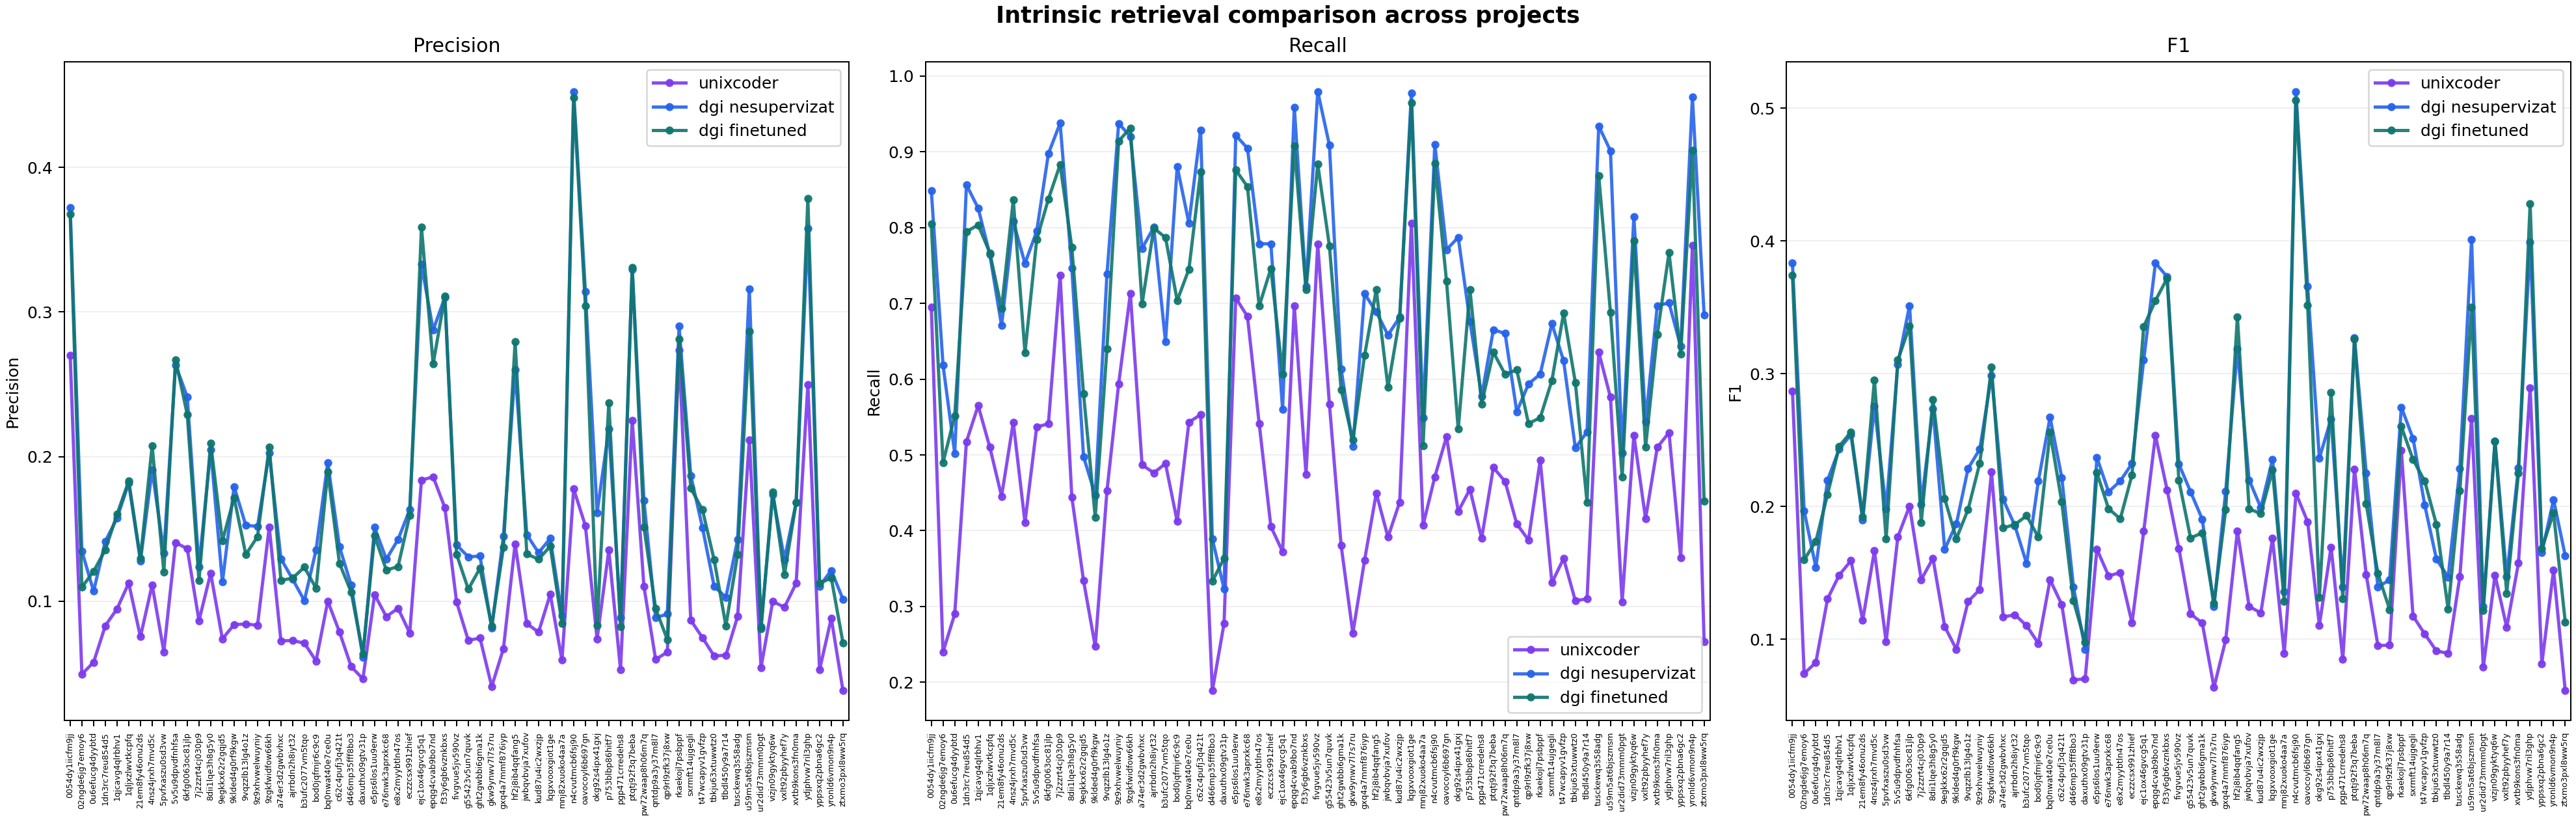
\includegraphics[width=0.95\textwidth]{intrinsic_retrieval_connected_dots.png}
    \caption{Evaluarea intrinsecă a recuperării de noduri prin compararea vecinătății structurale cu nodurile apropiate în spațiul de embedding}
    \label{fig:intrinsic-retrieval-connected-dots}
\end{figure}

\begin{flushleft}
\small
\setlength{\tabcolsep}{6pt}
\renewcommand{\arraystretch}{0.95}
\captionsetup{type=table,hypcap=false,justification=raggedright,singlelinecheck=false}
\caption{Evaluarea intrinsecă: media metricilor de recuperare la nivel de proiecte}
\label{tab:intrinsic-retrieval-mean-projects}
\begin{tabular}{lccc}
\toprule
\textbf{Metodă} & \textbf{Precision} & \textbf{Recall} & \textbf{F1} \\
\midrule
UniXcoder & 0.102 & 0.472 & 0.140 \\
DGI nesupervizat & \textbf{0.172} & \textbf{0.724} & \textbf{0.233} \\
DGI finetuned & 0.167 & 0.688 & 0.224 \\
\bottomrule
\end{tabular}
\end{flushleft}

\clearpage
\subsection*{Evaluarea recuperării de noduri în mod extrinsec}
\addcontentsline{toc}{subsection}{Evaluarea recuperării de noduri în mod extrinsec}
\label{anexa:evaluare-extrinseca}

\begin{figure}[htbp]
    \centering
    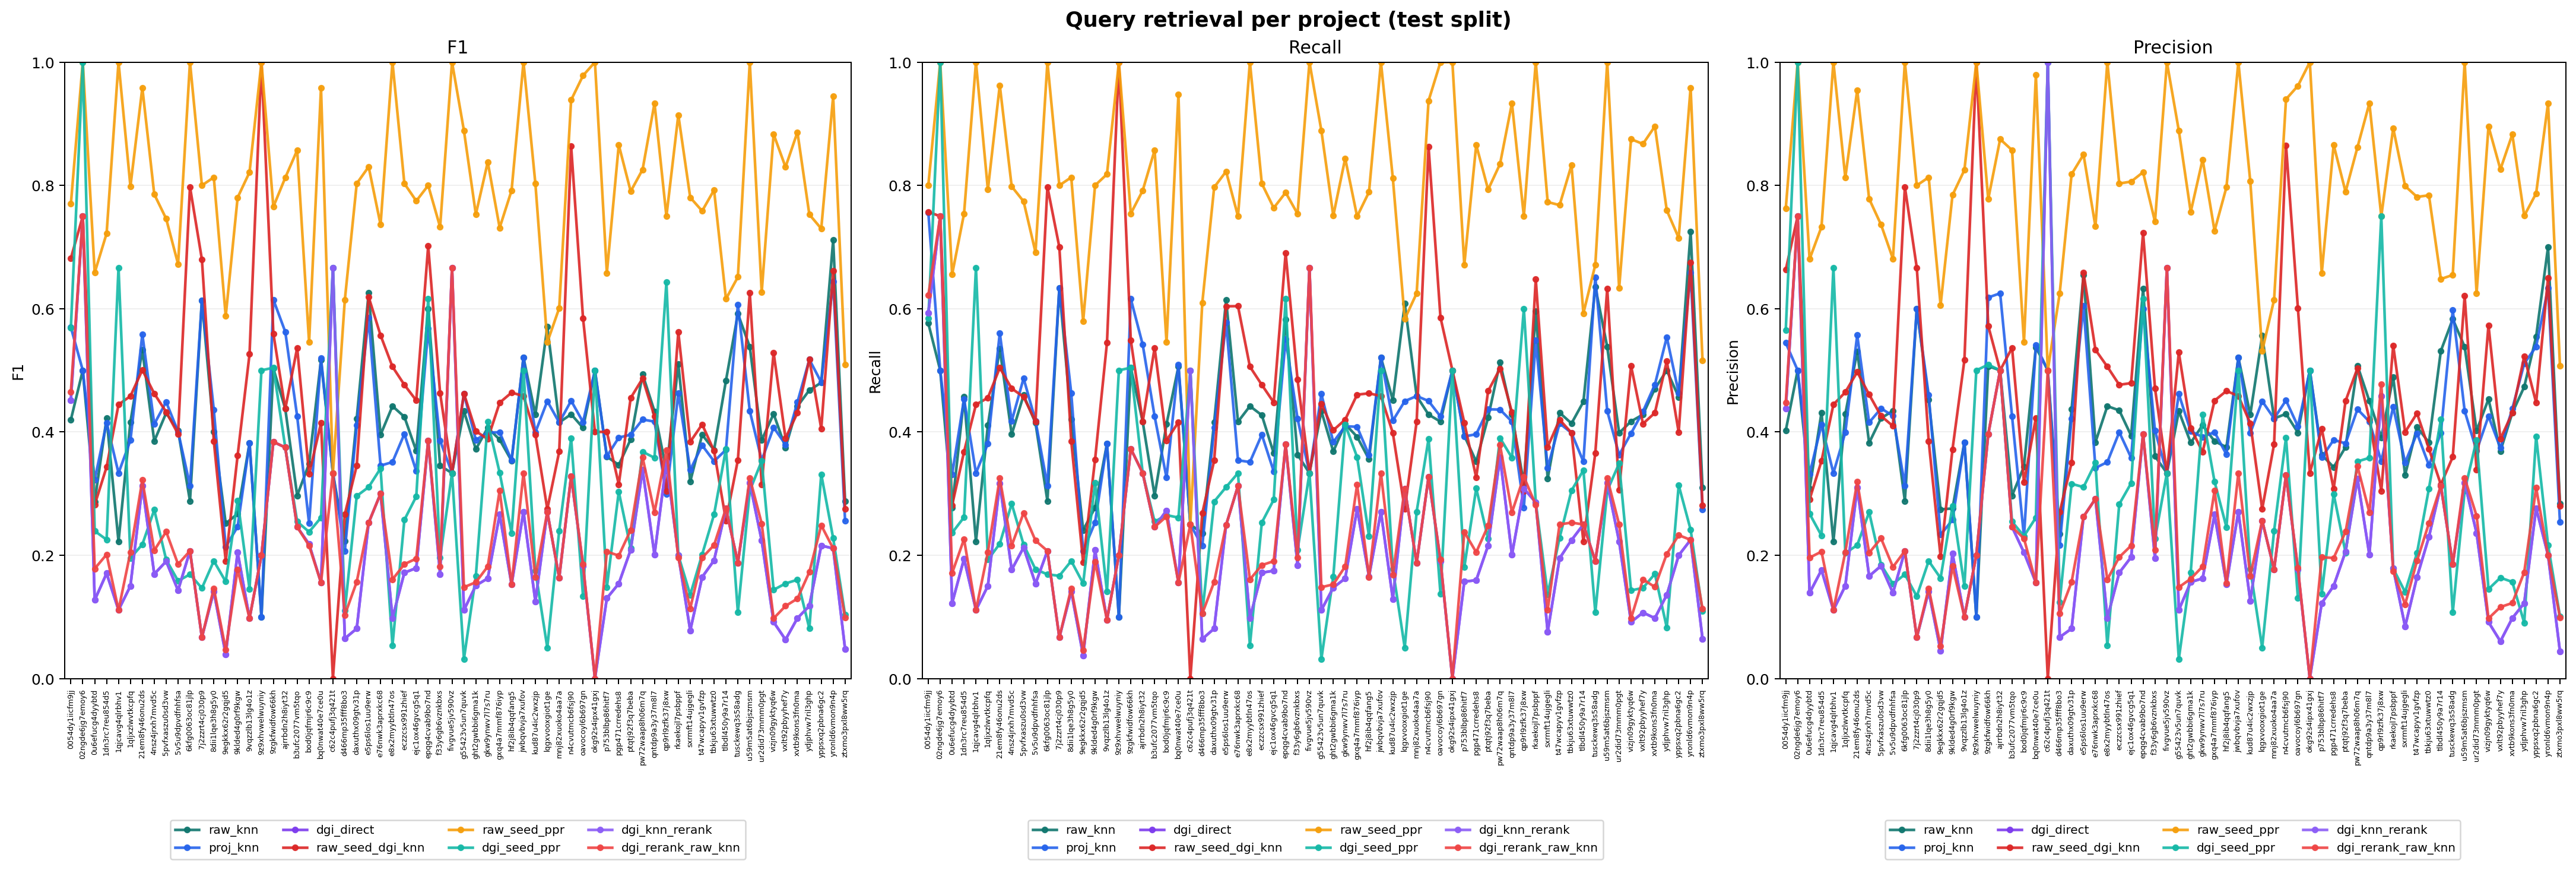
\includegraphics[width=0.95\textwidth]{retrieval_evaluation_inductive_test_per_project.png}
    \caption{Evaluarea extrinsecă a recuperării de noduri pe split-ul de test pentru metodele condiționate de interogări în limbaj natural}
    \label{fig:extrinsic-retrieval-inductive-test}
\end{figure}


\begin{flushleft}
\small
\setlength{\tabcolsep}{4pt}
\renewcommand{\arraystretch}{0.95}
\captionsetup{type=table,hypcap=false,justification=raggedright,singlelinecheck=false}
\caption{Evaluarea extrinsecă: metrici de recuperare pentru vecinătatea la un salt}
\label{tab:extrinsic-retrieval-one-hop}
\begin{tabular}{lccc}
\toprule
\textbf{Metodă} & \textbf{F1} & \textbf{Recall} & \textbf{Precision} \\
\midrule
\texttt{raw\_knn} & 0.392 $\pm$ 0.232 & 0.406 $\pm$ 0.246 & 0.401 $\pm$ 0.240 \\
\texttt{proj\_knn} & 0.387 $\pm$ 0.231 & 0.403 $\pm$ 0.246 & 0.394 $\pm$ 0.235 \\
\texttt{dgi\_direct} & 0.163 $\pm$ 0.248 & 0.173 $\pm$ 0.264 & 0.168 $\pm$ 0.258 \\
\texttt{raw\_seed\_dgi\_knn} & 0.415 $\pm$ 0.294 & 0.423 $\pm$ 0.297 & 0.424 $\pm$ 0.306 \\
\texttt{raw\_seed\_ppr} & \textbf{0.758 $\pm$ 0.388} & \textbf{0.765 $\pm$ 0.387} & \textbf{0.765 $\pm$ 0.386} \\
\texttt{dgi\_seed\_ppr} & 0.226 $\pm$ 0.328 & 0.233 $\pm$ 0.338 & 0.234 $\pm$ 0.339 \\
\texttt{dgi\_knn\_rerank} & 0.163 $\pm$ 0.248 & 0.173 $\pm$ 0.264 & 0.168 $\pm$ 0.258 \\
\texttt{dgi\_rerank\_raw\_knn} & 0.192 $\pm$ 0.252 & 0.204 $\pm$ 0.270 & 0.197 $\pm$ 0.262 \\
\bottomrule
\end{tabular}
\end{flushleft}

\vspace{-0.75em}
\begin{flushleft}
\small
\setlength{\tabcolsep}{4pt}
\renewcommand{\arraystretch}{0.95}
\captionsetup{type=table,hypcap=false,justification=raggedright,singlelinecheck=false}
\caption{Evaluarea extrinsecă: metrici de ranking MRR și Hits@k}
\label{tab:extrinsic-ranking-metrics}
\begin{tabular}{lcccc}
\toprule
\textbf{Metodă} & \textbf{MRR} & \textbf{Hits@1} & \textbf{Hits@5} & \textbf{Hits@10} \\
\midrule
\texttt{raw\_knn} & 0.750 $\pm$ 0.361 & 0.646 & \textbf{0.882} & \textbf{0.894} \\
\texttt{proj\_knn} & \textbf{0.757 $\pm$ 0.363} & \textbf{0.663} & 0.880 & 0.889 \\
\texttt{dgi\_direct} & 0.140 $\pm$ 0.296 & 0.086 & 0.204 & 0.246 \\
\texttt{raw\_seed\_dgi\_knn} & 0.694 $\pm$ 0.439 & 0.661 & 0.738 & 0.757 \\
\texttt{raw\_seed\_ppr} & 0.616 $\pm$ 0.421 & 0.504 & 0.742 & 0.756 \\
\texttt{dgi\_seed\_ppr} & 0.112 $\pm$ 0.272 & 0.070 & 0.166 & 0.189 \\
\texttt{dgi\_knn\_rerank} & 0.140 $\pm$ 0.296 & 0.086 & 0.204 & 0.246 \\
\texttt{dgi\_rerank\_raw\_knn} & 0.175 $\pm$ 0.315 & 0.101 & 0.272 & 0.316 \\
\bottomrule
\end{tabular}
\end{flushleft}

\vspace{-0.75em}
\begin{flushleft}
\small
\setlength{\tabcolsep}{5pt}
\renewcommand{\arraystretch}{0.95}
\captionsetup{type=table,hypcap=false,justification=raggedright,singlelinecheck=false}
\caption{Evaluarea extrinsecă: relevanța semantică medie față de interogare, calculată prin similaritate cosinus în spațiul UniXcoder brut}
\label{tab:extrinsic-semantic-relevance}
\begin{tabular}{lc}
\toprule
\textbf{Metodă} & \textbf{Medie $\pm$ deviație standard} \\
\midrule
\texttt{raw\_knn} & \textbf{0.444 $\pm$ 0.086} \\
\texttt{proj\_knn} & 0.427 $\pm$ 0.092 \\
\texttt{dgi\_direct} & 0.276 $\pm$ 0.101 \\
\texttt{raw\_seed\_dgi\_knn} & 0.349 $\pm$ 0.103 \\
\texttt{raw\_seed\_ppr} & 0.345 $\pm$ 0.100 \\
\texttt{dgi\_seed\_ppr} & 0.253 $\pm$ 0.102 \\
\texttt{dgi\_knn\_rerank} & 0.276 $\pm$ 0.101 \\
\texttt{dgi\_rerank\_raw\_knn} & 0.325 $\pm$ 0.087 \\
\bottomrule
\end{tabular}
\end{flushleft}

\clearpage
\subsection*{Evaluarea clusterizării}
\addcontentsline{toc}{subsection}{Evaluarea clusterizării}
\label{anexa:evaluare-clusterizare}

\begin{figure}[htbp]
    \centering
    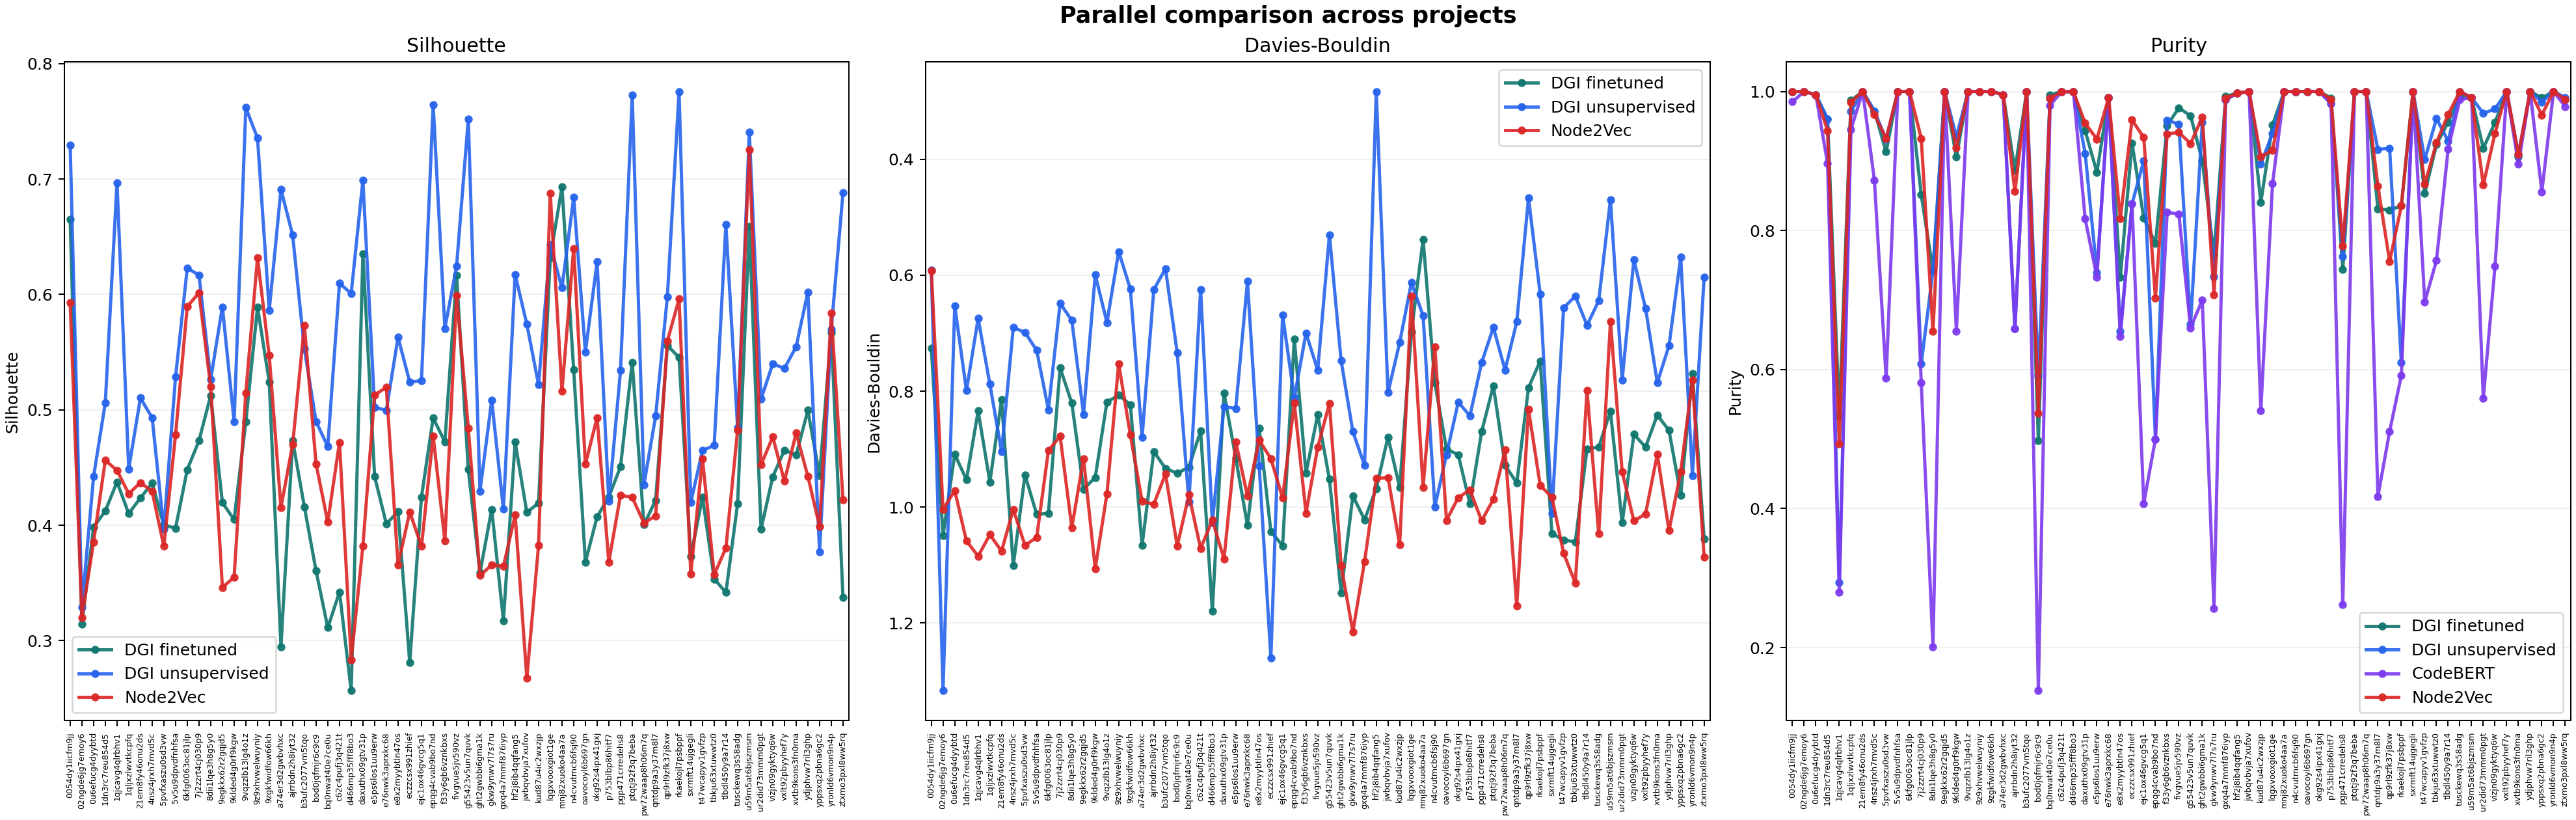
\includegraphics[width=0.95\textwidth]{clustering_comparison.png}
    \caption{Evaluarea clusterizării prin compararea reprezentărilor analizate în raport cu metricile Silhouette, Davies-Bouldin și puritate}
    \label{fig:clustering-comparison}
\end{figure}

\begin{flushleft}
\small
\setlength{\tabcolsep}{4pt}
\renewcommand{\arraystretch}{0.95}
\captionsetup{type=table,hypcap=false,justification=raggedright,singlelinecheck=false}
\caption{Evaluarea clusterizării}
\label{tab:clustering-evaluation-metrics}
\begin{tabular}{lccc}
\toprule
\textbf{Metodă} & \textbf{Silhouette} & \textbf{Davies-Bouldin} & \textbf{Puritate} \\
\midrule
DGI nesupervizat & \textbf{0.566 $\pm$ 0.107} & \textbf{0.741 $\pm$ 0.170} & 0.911 $\pm$ 0.147 \\
DGI finetuned & 0.445 $\pm$ 0.094 & 0.914 $\pm$ 0.116 & 0.931 $\pm$ 0.106 \\
Node2Vec & 0.457 $\pm$ 0.095 & 0.967 $\pm$ 0.121 & \textbf{0.932 $\pm$ 0.109} \\
CodeBERT & necalculat & necalculat & 0.814 $\pm$ 0.241 \\
\bottomrule
\end{tabular}
\end{flushleft}

\clearpage
\anexasection{Interfața aplicației}{anexa:interfata-aplicatie}

Această anexă include capturi din interfața aplicației, folosite pentru a ilustra componentele funcționale discutate în lucrare.

\begin{figure}[htbp]
    \centering
    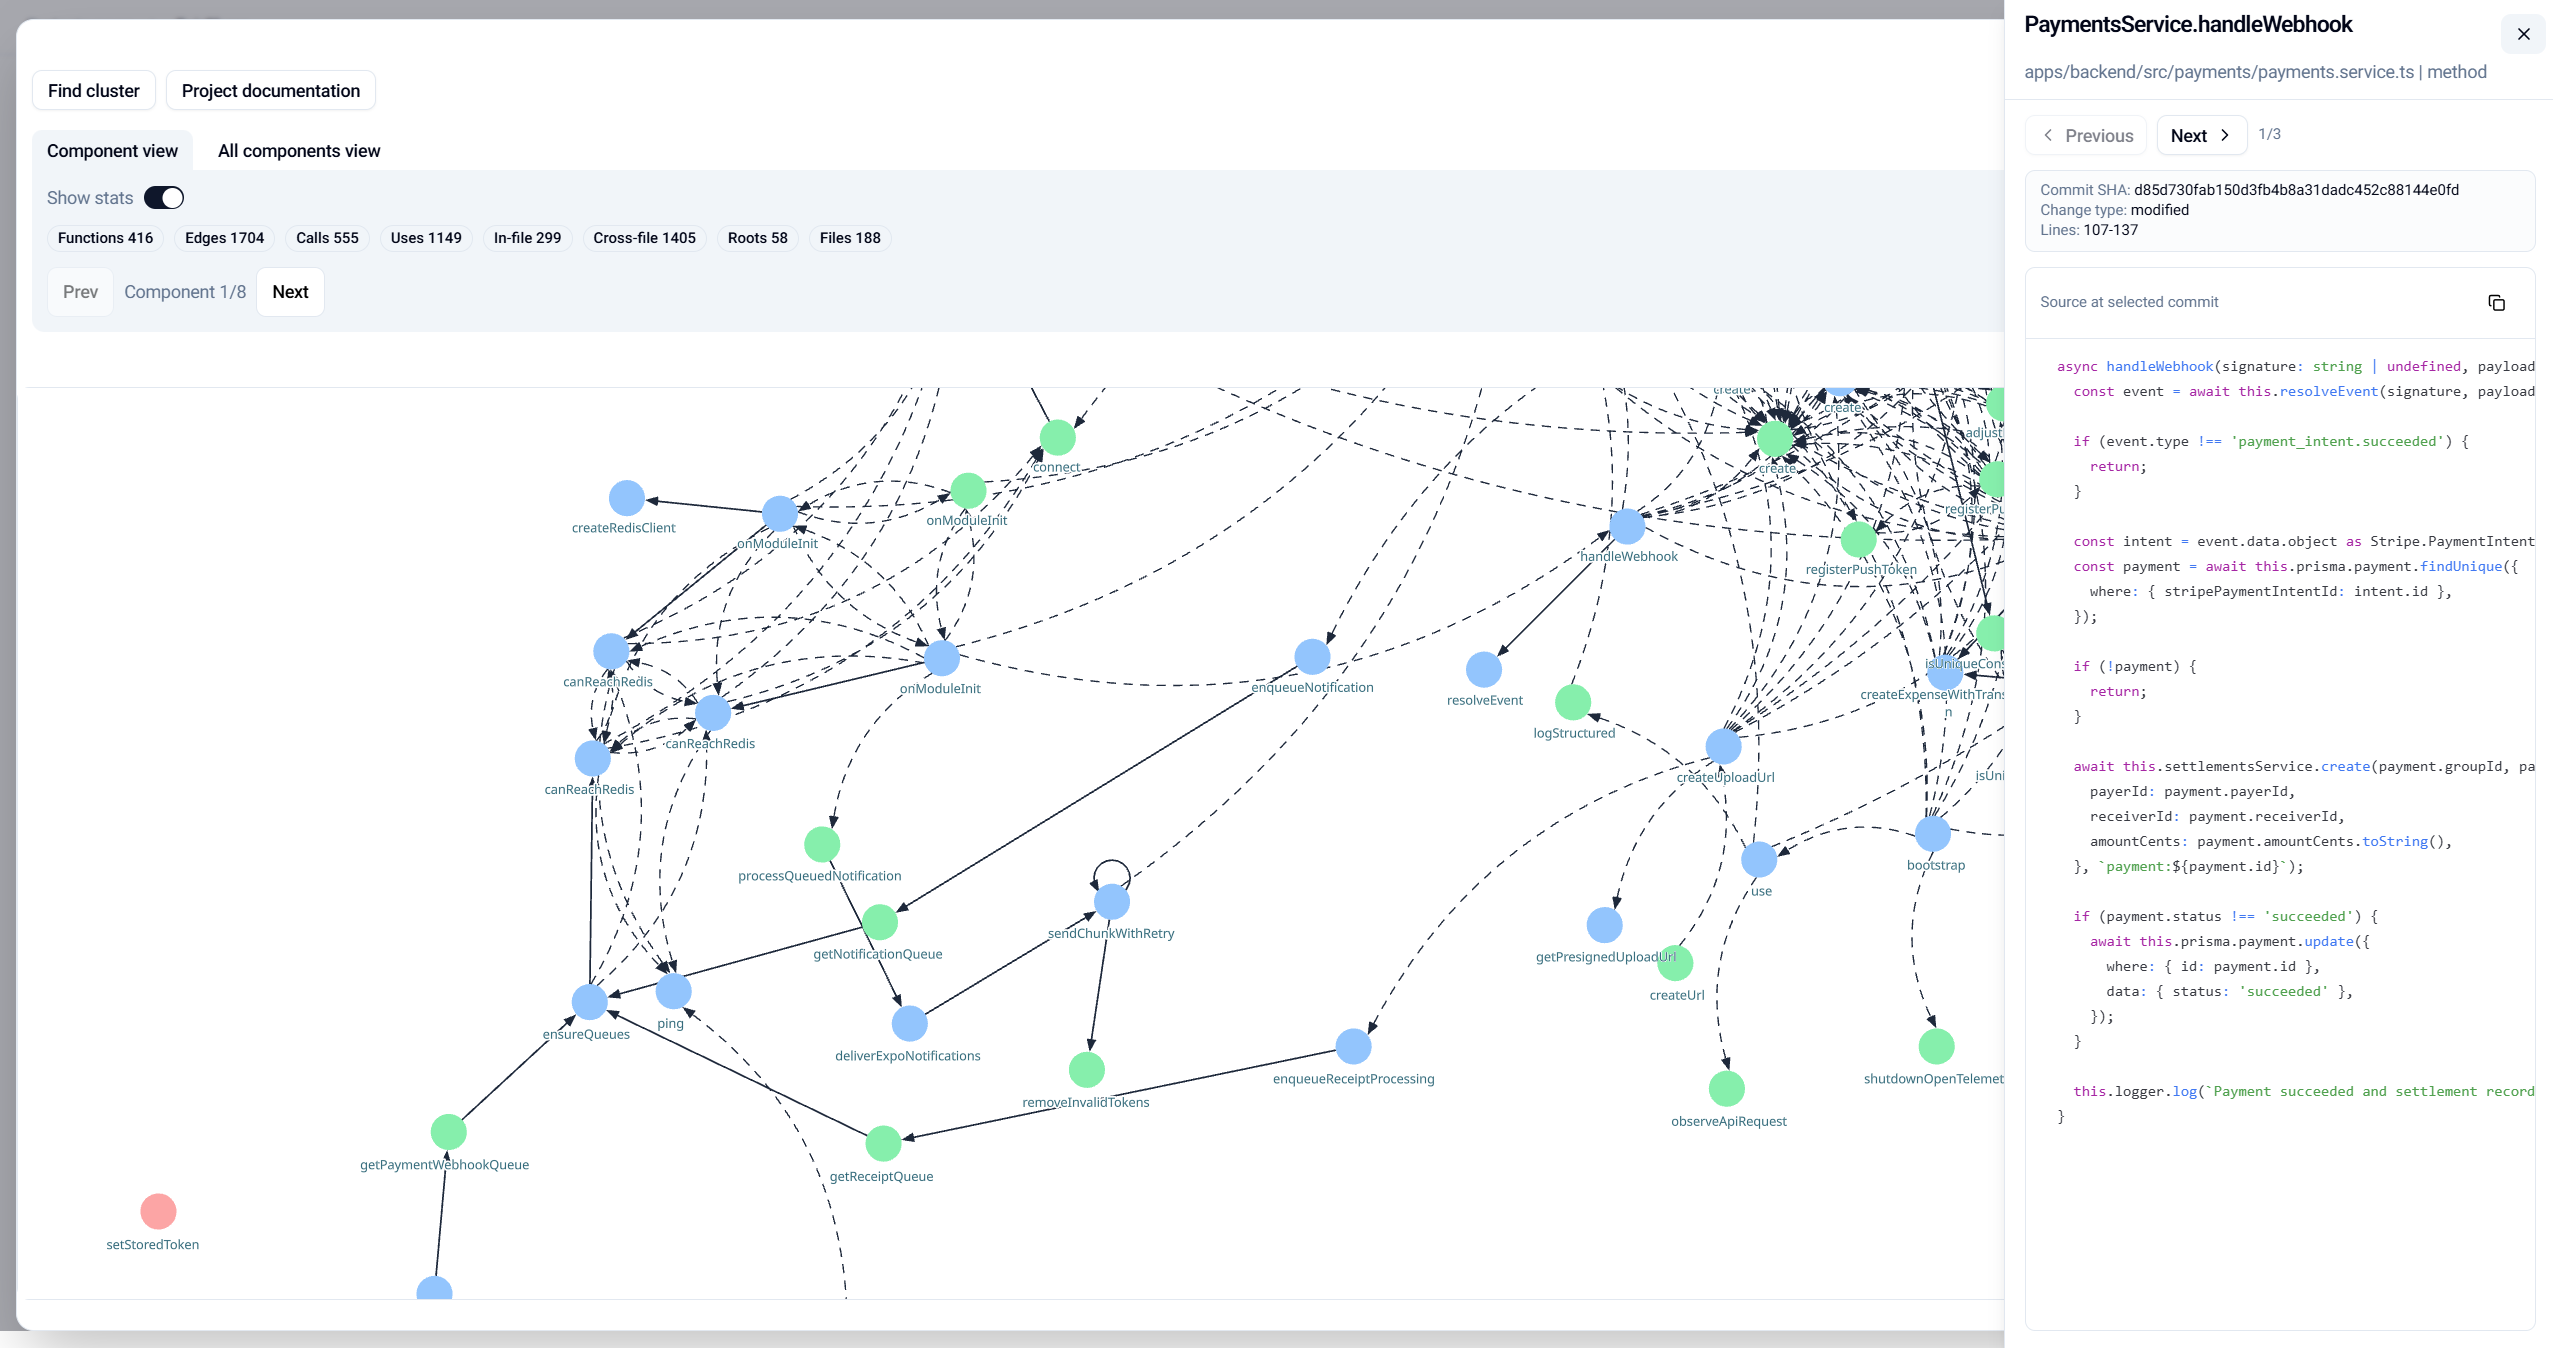
\includegraphics[width=0.95\textwidth]{knowledge-graph.png}
    \caption{Interfața aplicației pentru canvasul grafului de cunoștințe, unde nodurile și muchiile rezultate din analiza statică sunt afișate pentru explorarea structurii proiectului}
    \label{fig:knowledge-graph-interface}
\end{figure}

\begin{figure}[htbp]
    \centering
    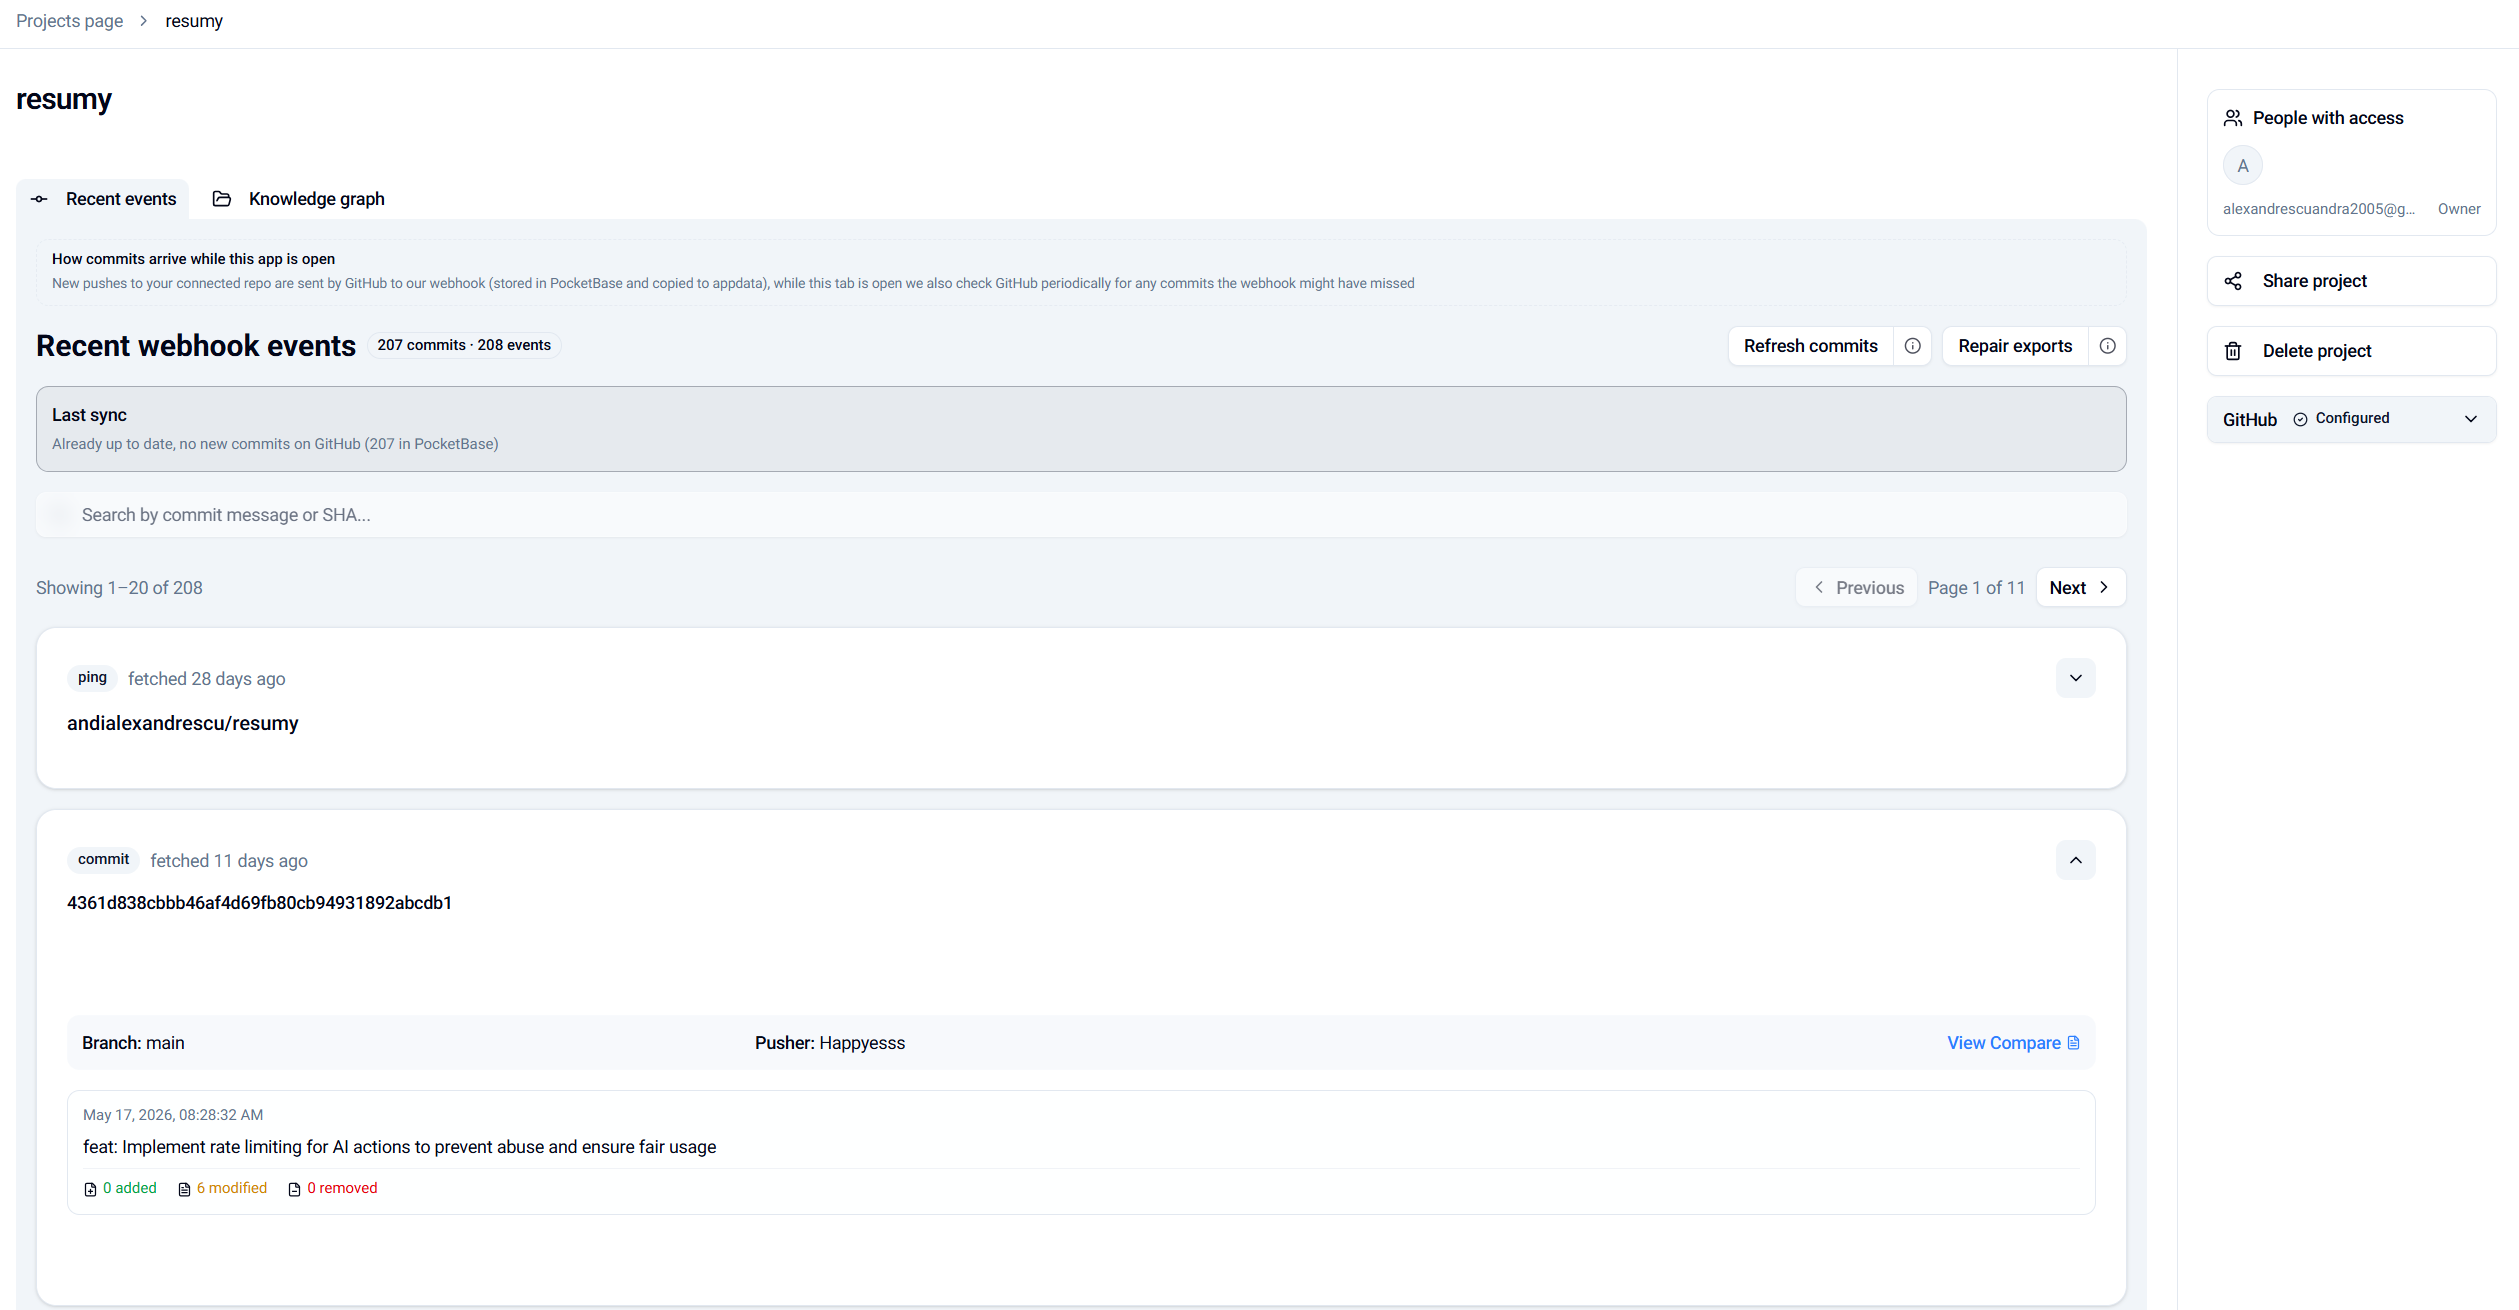
\includegraphics[width=0.95\textwidth]{webhook-events.png}
    \caption{Interfața aplicației pentru pagina evenimentelor webhook, unde sunt afișate evenimentele GitHub recepționate și sincronizate de sistem}
    \label{fig:webhook-events-interface}
\end{figure}

\begin{figure}[htbp]
    \centering
    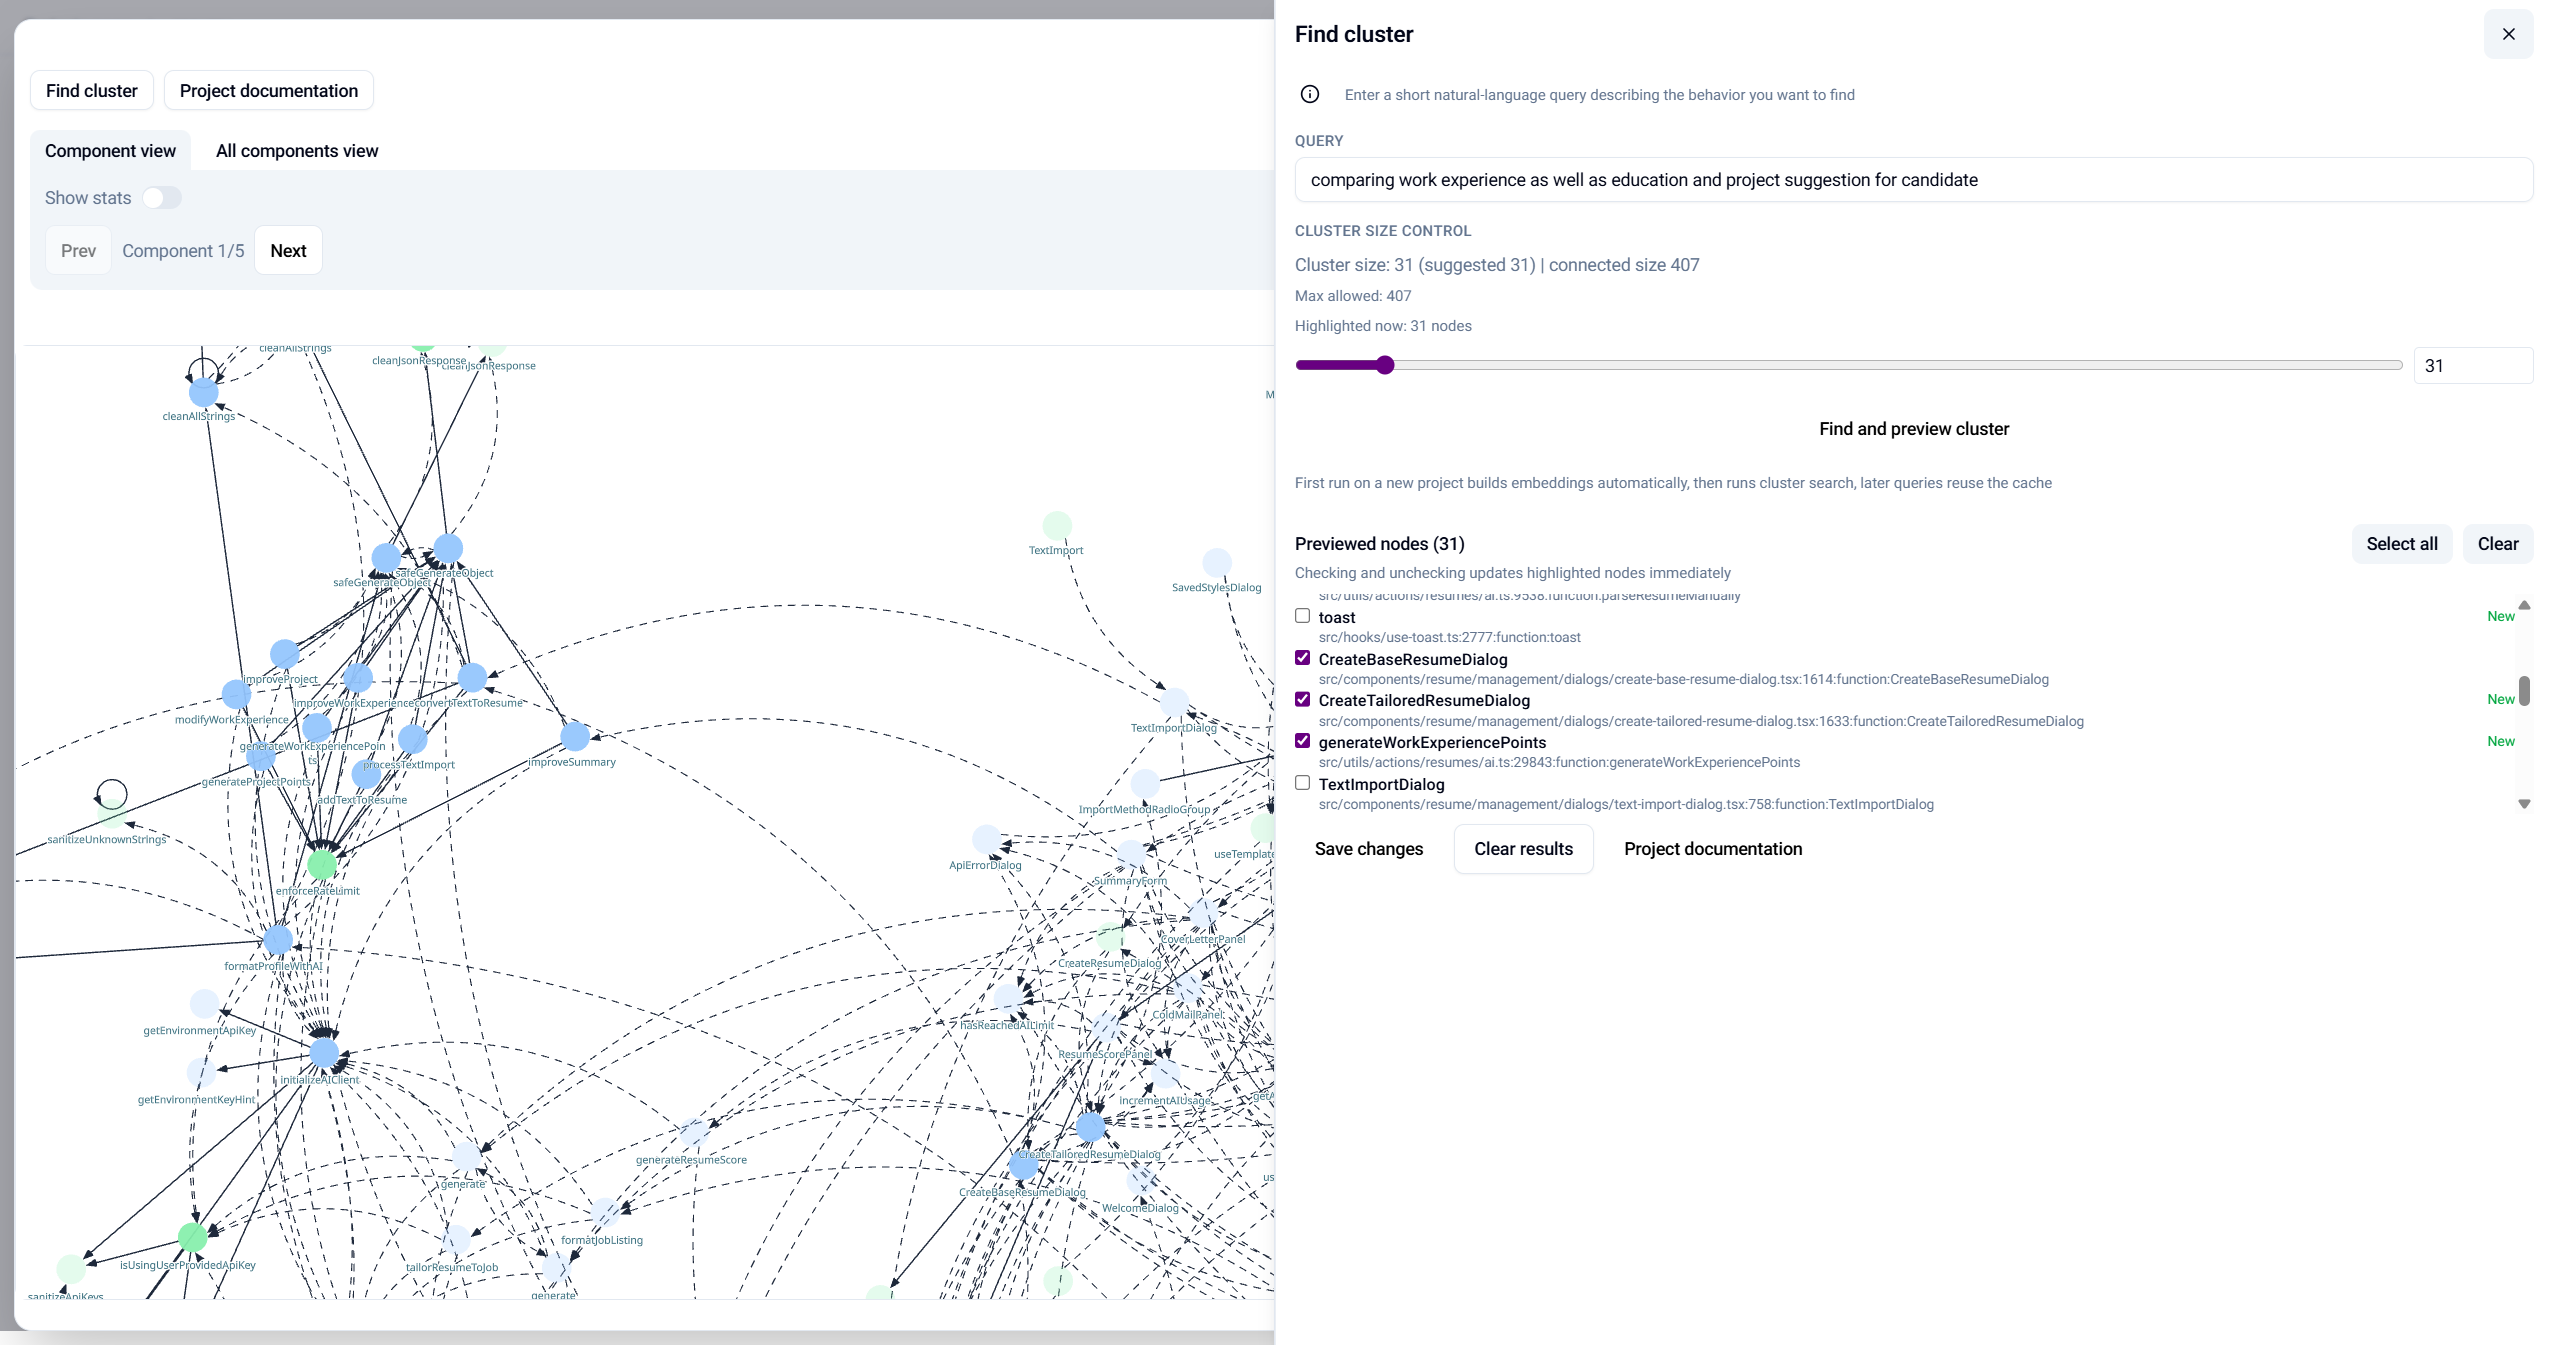
\includegraphics[width=0.95\textwidth]{find-cluster.png}
    \caption{Interfața aplicației pentru căutarea semantică de clustere prin PR, unde utilizatorul formulează interogarea și inspectează rezultatele relevante din graful de cunoștințe}
    \label{fig:find-cluster-interface}
\end{figure}

\begin{figure}[htbp]
    \centering
    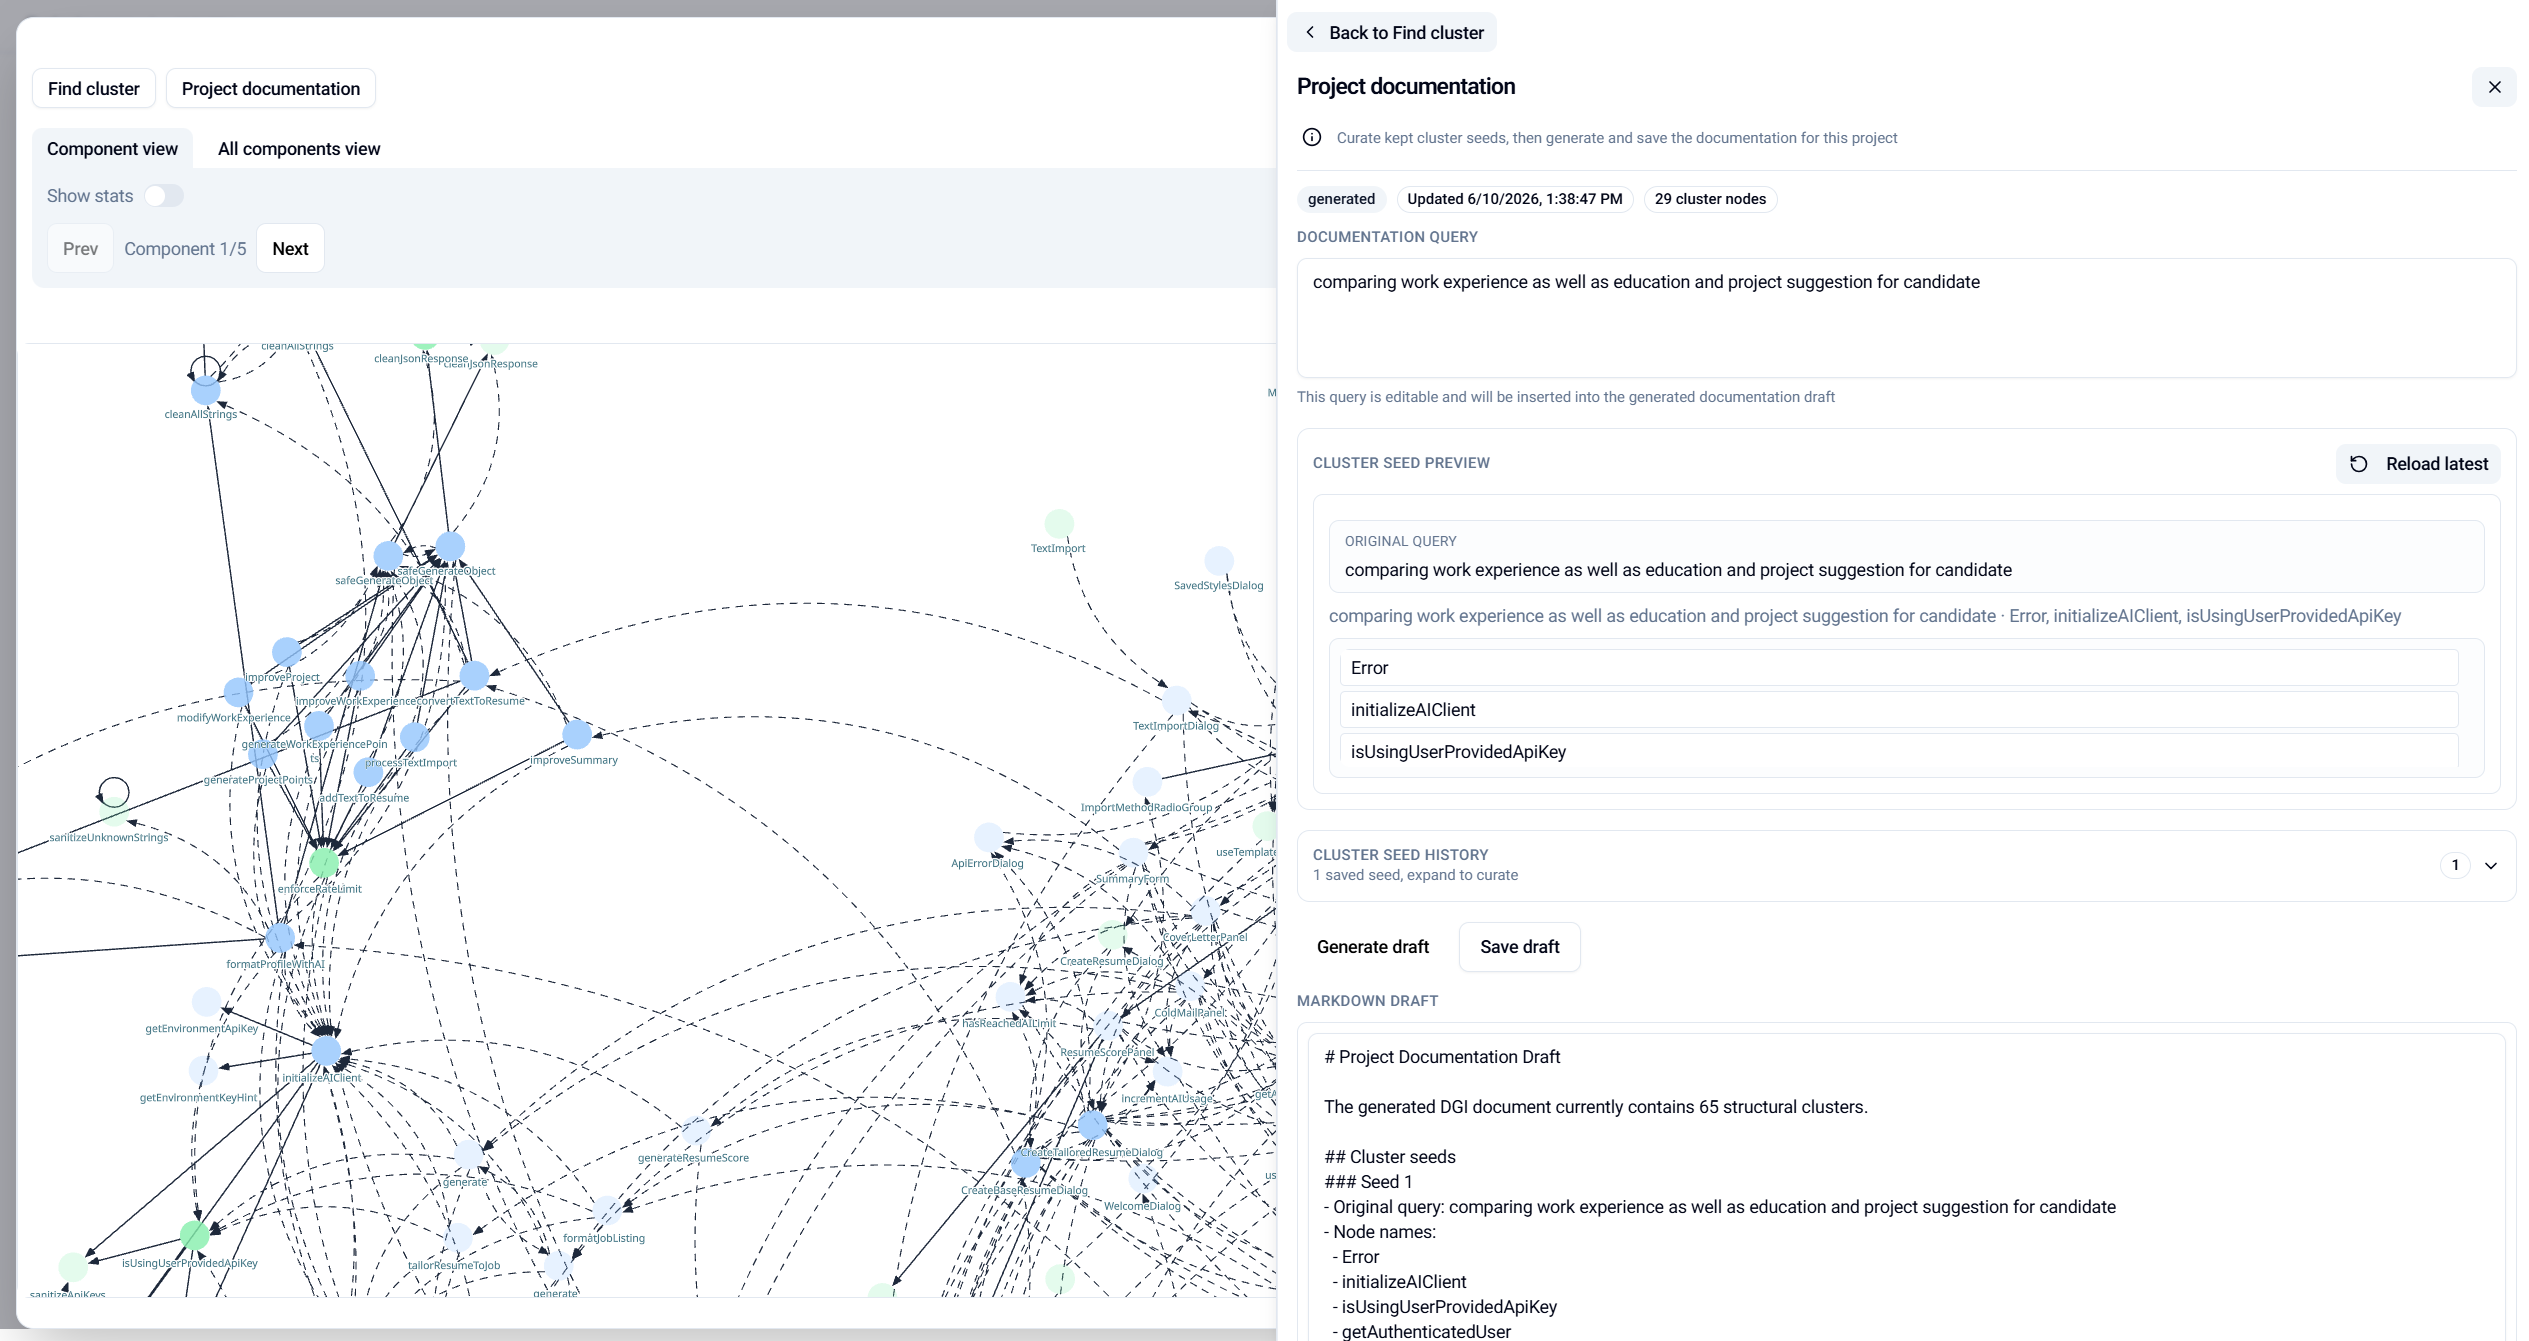
\includegraphics[width=0.95\textwidth]{project-documentation.png}
    \caption{Interfața aplicației pentru documentația proiectului, unde draft-ul structural generat pe baza clusterelor poate fi inspectat și editat de utilizator}
    \label{fig:project-documentation-interface}
\end{figure}

\end{document}